% Created by tikzDevice version 0.6.2-92-0ad2792 on 2013-03-06 20:16:19
% !TEX encoding = UTF-8 Unicode
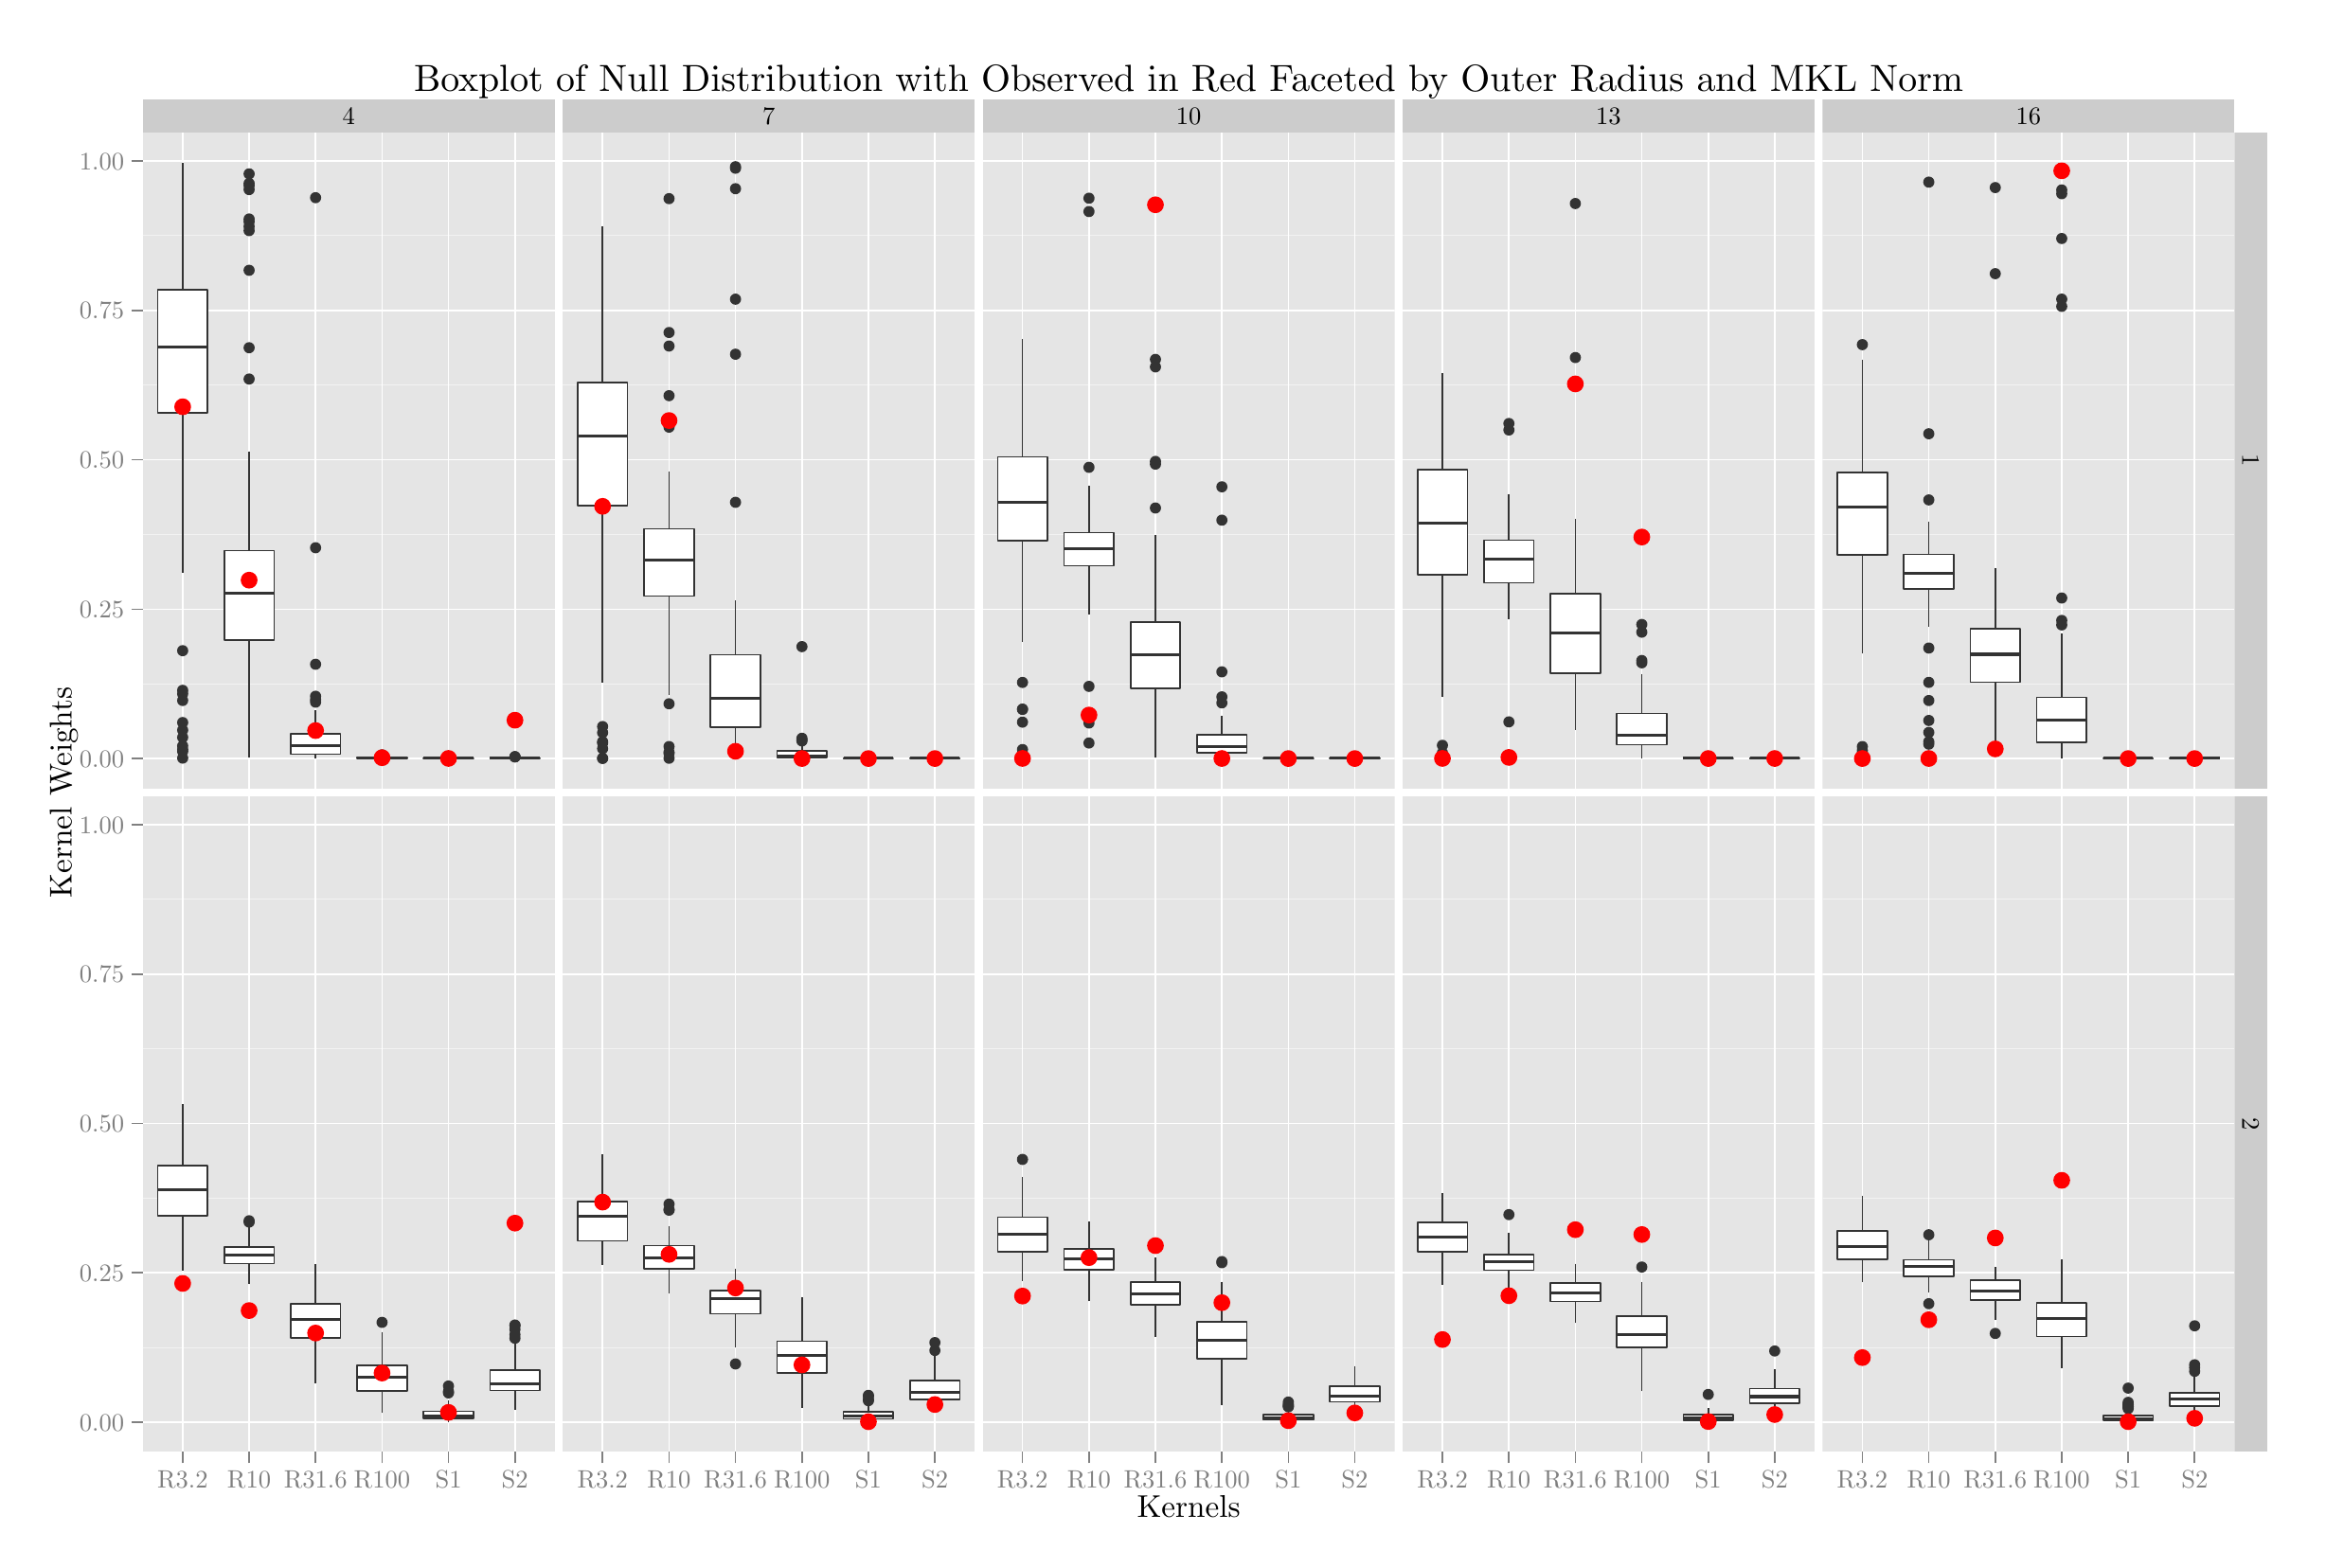
\begin{tikzpicture}[x=1pt,y=1pt]
\definecolor[named]{fillColor}{rgb}{1.00,1.00,1.00}
\path[use as bounding box,fill=fillColor,fill opacity=0.00] (0,0) rectangle (867.24,578.16);
\begin{scope}
\path[clip] (  0.00,  0.00) rectangle (867.24,578.16);
\definecolor[named]{drawColor}{rgb}{1.00,1.00,1.00}
\definecolor[named]{fillColor}{rgb}{1.00,1.00,1.00}

\path[draw=drawColor,line width= 0.6pt,line join=round,line cap=round,fill=fillColor] ( -0.00,  0.00) rectangle (867.24,578.16);
\end{scope}
\begin{scope}
\path[clip] ( 44.49,537.54) rectangle (201.69,550.17);
\definecolor[named]{fillColor}{rgb}{0.80,0.80,0.80}

\path[fill=fillColor] ( 44.49,537.54) rectangle (201.69,550.17);
\definecolor[named]{drawColor}{rgb}{0.00,0.00,0.00}

\node[text=drawColor,anchor=base,inner sep=0pt, outer sep=0pt, scale=  0.96] at (123.09,540.55) {4};
\end{scope}
\begin{scope}
\path[clip] (204.70,537.54) rectangle (361.91,550.17);
\definecolor[named]{fillColor}{rgb}{0.80,0.80,0.80}

\path[fill=fillColor] (204.70,537.54) rectangle (361.91,550.17);
\definecolor[named]{drawColor}{rgb}{0.00,0.00,0.00}

\node[text=drawColor,anchor=base,inner sep=0pt, outer sep=0pt, scale=  0.96] at (283.31,540.55) {7};
\end{scope}
\begin{scope}
\path[clip] (364.92,537.54) rectangle (522.13,550.17);
\definecolor[named]{fillColor}{rgb}{0.80,0.80,0.80}

\path[fill=fillColor] (364.92,537.54) rectangle (522.13,550.17);
\definecolor[named]{drawColor}{rgb}{0.00,0.00,0.00}

\node[text=drawColor,anchor=base,inner sep=0pt, outer sep=0pt, scale=  0.96] at (443.52,540.55) {10};
\end{scope}
\begin{scope}
\path[clip] (525.14,537.54) rectangle (682.34,550.17);
\definecolor[named]{fillColor}{rgb}{0.80,0.80,0.80}

\path[fill=fillColor] (525.14,537.54) rectangle (682.34,550.17);
\definecolor[named]{drawColor}{rgb}{0.00,0.00,0.00}

\node[text=drawColor,anchor=base,inner sep=0pt, outer sep=0pt, scale=  0.96] at (603.74,540.55) {13};
\end{scope}
\begin{scope}
\path[clip] (685.35,537.54) rectangle (842.56,550.17);
\definecolor[named]{fillColor}{rgb}{0.80,0.80,0.80}

\path[fill=fillColor] (685.35,537.54) rectangle (842.56,550.17);
\definecolor[named]{drawColor}{rgb}{0.00,0.00,0.00}

\node[text=drawColor,anchor=base,inner sep=0pt, outer sep=0pt, scale=  0.96] at (763.96,540.55) {16};
\end{scope}
\begin{scope}
\path[clip] ( 44.49,287.29) rectangle (201.69,537.54);
\definecolor[named]{fillColor}{rgb}{0.90,0.90,0.90}

\path[fill=fillColor] ( 44.49,287.29) rectangle (201.69,537.54);
\definecolor[named]{drawColor}{rgb}{0.95,0.95,0.95}

\path[draw=drawColor,line width= 0.3pt,line join=round] ( 44.49,327.17) --
	(201.69,327.17);

\path[draw=drawColor,line width= 0.3pt,line join=round] ( 44.49,384.18) --
	(201.69,384.18);

\path[draw=drawColor,line width= 0.3pt,line join=round] ( 44.49,441.20) --
	(201.69,441.20);

\path[draw=drawColor,line width= 0.3pt,line join=round] ( 44.49,498.21) --
	(201.69,498.21);
\definecolor[named]{drawColor}{rgb}{1.00,1.00,1.00}

\path[draw=drawColor,line width= 0.6pt,line join=round] ( 44.49,298.67) --
	(201.69,298.67);

\path[draw=drawColor,line width= 0.6pt,line join=round] ( 44.49,355.68) --
	(201.69,355.68);

\path[draw=drawColor,line width= 0.6pt,line join=round] ( 44.49,412.69) --
	(201.69,412.69);

\path[draw=drawColor,line width= 0.6pt,line join=round] ( 44.49,469.70) --
	(201.69,469.70);

\path[draw=drawColor,line width= 0.6pt,line join=round] ( 44.49,526.72) --
	(201.69,526.72);

\path[draw=drawColor,line width= 0.6pt,line join=round] ( 59.70,287.29) --
	( 59.70,537.54);

\path[draw=drawColor,line width= 0.6pt,line join=round] ( 85.05,287.29) --
	( 85.05,537.54);

\path[draw=drawColor,line width= 0.6pt,line join=round] (110.41,287.29) --
	(110.41,537.54);

\path[draw=drawColor,line width= 0.6pt,line join=round] (135.77,287.29) --
	(135.77,537.54);

\path[draw=drawColor,line width= 0.6pt,line join=round] (161.12,287.29) --
	(161.12,537.54);

\path[draw=drawColor,line width= 0.6pt,line join=round] (186.48,287.29) --
	(186.48,537.54);
\definecolor[named]{fillColor}{rgb}{0.20,0.20,0.20}

\path[fill=fillColor] ( 59.70,301.39) circle (  2.13);

\path[fill=fillColor] ( 59.70,320.83) circle (  2.13);

\path[fill=fillColor] ( 59.70,309.52) circle (  2.13);

\path[fill=fillColor] ( 59.70,312.41) circle (  2.13);

\path[fill=fillColor] ( 59.70,324.70) circle (  2.13);

\path[fill=fillColor] ( 59.70,303.50) circle (  2.13);

\path[fill=fillColor] ( 59.70,302.12) circle (  2.13);

\path[fill=fillColor] ( 59.70,323.35) circle (  2.13);

\path[fill=fillColor] ( 59.70,339.84) circle (  2.13);

\path[fill=fillColor] ( 59.70,306.75) circle (  2.13);

\path[fill=fillColor] ( 59.70,298.84) circle (  2.13);
\definecolor[named]{drawColor}{rgb}{0.20,0.20,0.20}

\path[draw=drawColor,line width= 0.6pt,line join=round,fill=fillColor] ( 59.70,477.67) -- ( 59.70,526.17);

\path[draw=drawColor,line width= 0.6pt,line join=round,fill=fillColor] ( 59.70,430.69) -- ( 59.70,369.63);
\definecolor[named]{fillColor}{rgb}{1.00,1.00,1.00}

\path[draw=drawColor,line width= 0.6pt,line join=round,line cap=round,fill=fillColor] ( 50.19,477.67) --
	( 50.19,430.69) --
	( 69.21,430.69) --
	( 69.21,477.67) --
	( 50.19,477.67) --
	cycle;
\definecolor[named]{fillColor}{rgb}{0.20,0.20,0.20}

\path[draw=drawColor,line width= 1.1pt,line join=round,fill=fillColor] ( 50.19,455.68) -- ( 69.21,455.68);

\path[fill=fillColor] ( 85.05,443.51) circle (  2.13);

\path[fill=fillColor] ( 85.05,503.57) circle (  2.13);

\path[fill=fillColor] ( 85.05,515.80) circle (  2.13);

\path[fill=fillColor] ( 85.05,504.58) circle (  2.13);

\path[fill=fillColor] ( 85.05,500.14) circle (  2.13);

\path[fill=fillColor] ( 85.05,521.79) circle (  2.13);

\path[fill=fillColor] ( 85.05,517.38) circle (  2.13);

\path[fill=fillColor] ( 85.05,501.71) circle (  2.13);

\path[fill=fillColor] ( 85.05,485.00) circle (  2.13);

\path[fill=fillColor] ( 85.05,518.17) circle (  2.13);

\path[fill=fillColor] ( 85.05,455.45) circle (  2.13);

\path[draw=drawColor,line width= 0.6pt,line join=round,fill=fillColor] ( 85.05,378.02) -- ( 85.05,415.89);

\path[draw=drawColor,line width= 0.6pt,line join=round,fill=fillColor] ( 85.05,343.91) -- ( 85.05,299.20);
\definecolor[named]{fillColor}{rgb}{1.00,1.00,1.00}

\path[draw=drawColor,line width= 0.6pt,line join=round,line cap=round,fill=fillColor] ( 75.55,378.02) --
	( 75.55,343.91) --
	( 94.56,343.91) --
	( 94.56,378.02) --
	( 75.55,378.02) --
	cycle;
\definecolor[named]{fillColor}{rgb}{0.20,0.20,0.20}

\path[draw=drawColor,line width= 1.1pt,line join=round,fill=fillColor] ( 75.55,361.64) -- ( 94.56,361.64);

\path[fill=fillColor] (110.41,320.19) circle (  2.13);

\path[fill=fillColor] (110.41,379.12) circle (  2.13);

\path[fill=fillColor] (110.41,322.45) circle (  2.13);

\path[fill=fillColor] (110.41,321.11) circle (  2.13);

\path[fill=fillColor] (110.41,512.71) circle (  2.13);

\path[fill=fillColor] (110.41,334.65) circle (  2.13);

\path[draw=drawColor,line width= 0.6pt,line join=round,fill=fillColor] (110.41,308.03) -- (110.41,317.12);

\path[draw=drawColor,line width= 0.6pt,line join=round,fill=fillColor] (110.41,300.34) -- (110.41,298.67);
\definecolor[named]{fillColor}{rgb}{1.00,1.00,1.00}

\path[draw=drawColor,line width= 0.6pt,line join=round,line cap=round,fill=fillColor] (100.90,308.03) --
	(100.90,300.34) --
	(119.92,300.34) --
	(119.92,308.03) --
	(100.90,308.03) --
	cycle;
\definecolor[named]{fillColor}{rgb}{0.20,0.20,0.20}

\path[draw=drawColor,line width= 1.1pt,line join=round,fill=fillColor] (100.90,303.42) -- (119.92,303.42);

\path[fill=fillColor] (135.77,299.50) circle (  2.13);

\path[fill=fillColor] (135.77,299.57) circle (  2.13);

\path[fill=fillColor] (135.77,299.61) circle (  2.13);

\path[fill=fillColor] (135.77,299.49) circle (  2.13);

\path[fill=fillColor] (135.77,300.09) circle (  2.13);

\path[draw=drawColor,line width= 0.6pt,line join=round,fill=fillColor] (135.77,299.02) -- (135.77,299.42);

\path[draw=drawColor,line width= 0.6pt,line join=round,fill=fillColor] (135.77,298.75) -- (135.77,298.67);
\definecolor[named]{fillColor}{rgb}{1.00,1.00,1.00}

\path[draw=drawColor,line width= 0.6pt,line join=round,line cap=round,fill=fillColor] (126.26,299.02) --
	(126.26,298.75) --
	(145.27,298.75) --
	(145.27,299.02) --
	(126.26,299.02) --
	cycle;
\definecolor[named]{fillColor}{rgb}{0.20,0.20,0.20}

\path[draw=drawColor,line width= 1.1pt,line join=round,fill=fillColor] (126.26,298.89) -- (145.27,298.89);

\path[fill=fillColor] (161.12,299.03) circle (  2.13);

\path[draw=drawColor,line width= 0.6pt,line join=round,fill=fillColor] (161.12,298.82) -- (161.12,298.97);

\path[draw=drawColor,line width= 0.6pt,line join=round,fill=fillColor] (161.12,298.69) -- (161.12,298.67);
\definecolor[named]{fillColor}{rgb}{1.00,1.00,1.00}

\path[draw=drawColor,line width= 0.6pt,line join=round,line cap=round,fill=fillColor] (151.61,298.82) --
	(151.61,298.69) --
	(170.63,298.69) --
	(170.63,298.82) --
	(151.61,298.82) --
	cycle;
\definecolor[named]{fillColor}{rgb}{0.20,0.20,0.20}

\path[draw=drawColor,line width= 1.1pt,line join=round,fill=fillColor] (151.61,298.75) -- (170.63,298.75);

\path[fill=fillColor] (186.48,299.30) circle (  2.13);

\path[fill=fillColor] (186.48,299.32) circle (  2.13);

\path[fill=fillColor] (186.48,299.41) circle (  2.13);

\path[draw=drawColor,line width= 0.6pt,line join=round,fill=fillColor] (186.48,298.92) -- (186.48,299.24);

\path[draw=drawColor,line width= 0.6pt,line join=round,fill=fillColor] (186.48,298.70) -- (186.48,298.67);
\definecolor[named]{fillColor}{rgb}{1.00,1.00,1.00}

\path[draw=drawColor,line width= 0.6pt,line join=round,line cap=round,fill=fillColor] (176.97,298.92) --
	(176.97,298.70) --
	(195.99,298.70) --
	(195.99,298.92) --
	(176.97,298.92) --
	cycle;
\definecolor[named]{fillColor}{rgb}{0.20,0.20,0.20}

\path[draw=drawColor,line width= 1.1pt,line join=round,fill=fillColor] (176.97,298.83) -- (195.99,298.83);
\definecolor[named]{fillColor}{rgb}{1.00,0.00,0.00}

\path[fill=fillColor] ( 59.70,432.91) circle (  3.20);

\path[fill=fillColor] ( 85.05,366.75) circle (  3.20);

\path[fill=fillColor] (110.41,309.35) circle (  3.20);

\path[fill=fillColor] (135.77,298.99) circle (  3.20);

\path[fill=fillColor] (161.12,298.72) circle (  3.20);

\path[fill=fillColor] (186.48,313.31) circle (  3.20);
\end{scope}
\begin{scope}
\path[clip] ( 44.49, 34.03) rectangle (201.69,284.28);
\definecolor[named]{fillColor}{rgb}{0.90,0.90,0.90}

\path[fill=fillColor] ( 44.49, 34.03) rectangle (201.69,284.28);
\definecolor[named]{drawColor}{rgb}{0.95,0.95,0.95}

\path[draw=drawColor,line width= 0.3pt,line join=round] ( 44.49, 73.91) --
	(201.69, 73.91);

\path[draw=drawColor,line width= 0.3pt,line join=round] ( 44.49,130.93) --
	(201.69,130.93);

\path[draw=drawColor,line width= 0.3pt,line join=round] ( 44.49,187.94) --
	(201.69,187.94);

\path[draw=drawColor,line width= 0.3pt,line join=round] ( 44.49,244.95) --
	(201.69,244.95);
\definecolor[named]{drawColor}{rgb}{1.00,1.00,1.00}

\path[draw=drawColor,line width= 0.6pt,line join=round] ( 44.49, 45.41) --
	(201.69, 45.41);

\path[draw=drawColor,line width= 0.6pt,line join=round] ( 44.49,102.42) --
	(201.69,102.42);

\path[draw=drawColor,line width= 0.6pt,line join=round] ( 44.49,159.43) --
	(201.69,159.43);

\path[draw=drawColor,line width= 0.6pt,line join=round] ( 44.49,216.44) --
	(201.69,216.44);

\path[draw=drawColor,line width= 0.6pt,line join=round] ( 44.49,273.46) --
	(201.69,273.46);

\path[draw=drawColor,line width= 0.6pt,line join=round] ( 59.70, 34.03) --
	( 59.70,284.28);

\path[draw=drawColor,line width= 0.6pt,line join=round] ( 85.05, 34.03) --
	( 85.05,284.28);

\path[draw=drawColor,line width= 0.6pt,line join=round] (110.41, 34.03) --
	(110.41,284.28);

\path[draw=drawColor,line width= 0.6pt,line join=round] (135.77, 34.03) --
	(135.77,284.28);

\path[draw=drawColor,line width= 0.6pt,line join=round] (161.12, 34.03) --
	(161.12,284.28);

\path[draw=drawColor,line width= 0.6pt,line join=round] (186.48, 34.03) --
	(186.48,284.28);
\definecolor[named]{drawColor}{rgb}{0.20,0.20,0.20}
\definecolor[named]{fillColor}{rgb}{0.20,0.20,0.20}

\path[draw=drawColor,line width= 0.6pt,line join=round,fill=fillColor] ( 59.70,143.26) -- ( 59.70,166.78);

\path[draw=drawColor,line width= 0.6pt,line join=round,fill=fillColor] ( 59.70,124.07) -- ( 59.70,103.19);
\definecolor[named]{fillColor}{rgb}{1.00,1.00,1.00}

\path[draw=drawColor,line width= 0.6pt,line join=round,line cap=round,fill=fillColor] ( 50.19,143.26) --
	( 50.19,124.07) --
	( 69.21,124.07) --
	( 69.21,143.26) --
	( 50.19,143.26) --
	cycle;
\definecolor[named]{fillColor}{rgb}{0.20,0.20,0.20}

\path[draw=drawColor,line width= 1.1pt,line join=round,fill=fillColor] ( 50.19,133.95) -- ( 69.21,133.95);

\path[fill=fillColor] ( 85.05,121.78) circle (  2.13);

\path[fill=fillColor] ( 85.05,122.28) circle (  2.13);

\path[draw=drawColor,line width= 0.6pt,line join=round,fill=fillColor] ( 85.05,112.19) -- ( 85.05,121.48);

\path[draw=drawColor,line width= 0.6pt,line join=round,fill=fillColor] ( 85.05,105.96) -- ( 85.05, 97.99);
\definecolor[named]{fillColor}{rgb}{1.00,1.00,1.00}

\path[draw=drawColor,line width= 0.6pt,line join=round,line cap=round,fill=fillColor] ( 75.55,112.19) --
	( 75.55,105.96) --
	( 94.56,105.96) --
	( 94.56,112.19) --
	( 75.55,112.19) --
	cycle;
\definecolor[named]{fillColor}{rgb}{0.20,0.20,0.20}

\path[draw=drawColor,line width= 1.1pt,line join=round,fill=fillColor] ( 75.55,109.29) -- ( 94.56,109.29);

\path[draw=drawColor,line width= 0.6pt,line join=round,fill=fillColor] (110.41, 90.46) -- (110.41,105.75);

\path[draw=drawColor,line width= 0.6pt,line join=round,fill=fillColor] (110.41, 77.48) -- (110.41, 60.37);
\definecolor[named]{fillColor}{rgb}{1.00,1.00,1.00}

\path[draw=drawColor,line width= 0.6pt,line join=round,line cap=round,fill=fillColor] (100.90, 90.46) --
	(100.90, 77.48) --
	(119.92, 77.48) --
	(119.92, 90.46) --
	(100.90, 90.46) --
	cycle;
\definecolor[named]{fillColor}{rgb}{0.20,0.20,0.20}

\path[draw=drawColor,line width= 1.1pt,line join=round,fill=fillColor] (100.90, 84.46) -- (119.92, 84.46);

\path[fill=fillColor] (135.77, 83.50) circle (  2.13);

\path[draw=drawColor,line width= 0.6pt,line join=round,fill=fillColor] (135.77, 67.15) -- (135.77, 79.90);

\path[draw=drawColor,line width= 0.6pt,line join=round,fill=fillColor] (135.77, 57.32) -- (135.77, 48.89);
\definecolor[named]{fillColor}{rgb}{1.00,1.00,1.00}

\path[draw=drawColor,line width= 0.6pt,line join=round,line cap=round,fill=fillColor] (126.26, 67.15) --
	(126.26, 57.32) --
	(145.27, 57.32) --
	(145.27, 67.15) --
	(126.26, 67.15) --
	cycle;
\definecolor[named]{fillColor}{rgb}{0.20,0.20,0.20}

\path[draw=drawColor,line width= 1.1pt,line join=round,fill=fillColor] (126.26, 62.69) -- (145.27, 62.69);

\path[fill=fillColor] (161.12, 59.21) circle (  2.13);

\path[fill=fillColor] (161.12, 56.58) circle (  2.13);

\path[fill=fillColor] (161.12, 57.09) circle (  2.13);

\path[draw=drawColor,line width= 0.6pt,line join=round,fill=fillColor] (161.12, 49.62) -- (161.12, 53.58);

\path[draw=drawColor,line width= 0.6pt,line join=round,fill=fillColor] (161.12, 46.75) -- (161.12, 45.54);
\definecolor[named]{fillColor}{rgb}{1.00,1.00,1.00}

\path[draw=drawColor,line width= 0.6pt,line join=round,line cap=round,fill=fillColor] (151.61, 49.62) --
	(151.61, 46.75) --
	(170.63, 46.75) --
	(170.63, 49.62) --
	(151.61, 49.62) --
	cycle;
\definecolor[named]{fillColor}{rgb}{0.20,0.20,0.20}

\path[draw=drawColor,line width= 1.1pt,line join=round,fill=fillColor] (151.61, 47.93) -- (170.63, 47.93);

\path[fill=fillColor] (186.48, 80.82) circle (  2.13);

\path[fill=fillColor] (186.48, 77.44) circle (  2.13);

\path[fill=fillColor] (186.48, 82.32) circle (  2.13);

\path[fill=fillColor] (186.48, 82.49) circle (  2.13);

\path[fill=fillColor] (186.48, 78.84) circle (  2.13);

\path[draw=drawColor,line width= 0.6pt,line join=round,fill=fillColor] (186.48, 65.40) -- (186.48, 76.86);

\path[draw=drawColor,line width= 0.6pt,line join=round,fill=fillColor] (186.48, 57.52) -- (186.48, 50.20);
\definecolor[named]{fillColor}{rgb}{1.00,1.00,1.00}

\path[draw=drawColor,line width= 0.6pt,line join=round,line cap=round,fill=fillColor] (176.97, 65.40) --
	(176.97, 57.52) --
	(195.99, 57.52) --
	(195.99, 65.40) --
	(176.97, 65.40) --
	cycle;
\definecolor[named]{fillColor}{rgb}{0.20,0.20,0.20}

\path[draw=drawColor,line width= 1.1pt,line join=round,fill=fillColor] (176.97, 59.91) -- (195.99, 59.91);
\definecolor[named]{fillColor}{rgb}{1.00,0.00,0.00}

\path[fill=fillColor] ( 59.70, 98.36) circle (  3.20);

\path[fill=fillColor] ( 85.05, 88.01) circle (  3.20);

\path[fill=fillColor] (110.41, 79.43) circle (  3.20);

\path[fill=fillColor] (135.77, 64.16) circle (  3.20);

\path[fill=fillColor] (161.12, 49.14) circle (  3.20);

\path[fill=fillColor] (186.48,121.38) circle (  3.20);
\end{scope}
\begin{scope}
\path[clip] (204.70,287.29) rectangle (361.91,537.54);
\definecolor[named]{fillColor}{rgb}{0.90,0.90,0.90}

\path[fill=fillColor] (204.70,287.29) rectangle (361.91,537.54);
\definecolor[named]{drawColor}{rgb}{0.95,0.95,0.95}

\path[draw=drawColor,line width= 0.3pt,line join=round] (204.70,327.17) --
	(361.91,327.17);

\path[draw=drawColor,line width= 0.3pt,line join=round] (204.70,384.18) --
	(361.91,384.18);

\path[draw=drawColor,line width= 0.3pt,line join=round] (204.70,441.20) --
	(361.91,441.20);

\path[draw=drawColor,line width= 0.3pt,line join=round] (204.70,498.21) --
	(361.91,498.21);
\definecolor[named]{drawColor}{rgb}{1.00,1.00,1.00}

\path[draw=drawColor,line width= 0.6pt,line join=round] (204.70,298.67) --
	(361.91,298.67);

\path[draw=drawColor,line width= 0.6pt,line join=round] (204.70,355.68) --
	(361.91,355.68);

\path[draw=drawColor,line width= 0.6pt,line join=round] (204.70,412.69) --
	(361.91,412.69);

\path[draw=drawColor,line width= 0.6pt,line join=round] (204.70,469.70) --
	(361.91,469.70);

\path[draw=drawColor,line width= 0.6pt,line join=round] (204.70,526.72) --
	(361.91,526.72);

\path[draw=drawColor,line width= 0.6pt,line join=round] (219.92,287.29) --
	(219.92,537.54);

\path[draw=drawColor,line width= 0.6pt,line join=round] (245.27,287.29) --
	(245.27,537.54);

\path[draw=drawColor,line width= 0.6pt,line join=round] (270.63,287.29) --
	(270.63,537.54);

\path[draw=drawColor,line width= 0.6pt,line join=round] (295.98,287.29) --
	(295.98,537.54);

\path[draw=drawColor,line width= 0.6pt,line join=round] (321.34,287.29) --
	(321.34,537.54);

\path[draw=drawColor,line width= 0.6pt,line join=round] (346.70,287.29) --
	(346.70,537.54);
\definecolor[named]{fillColor}{rgb}{0.20,0.20,0.20}

\path[fill=fillColor] (219.92,310.88) circle (  2.13);

\path[fill=fillColor] (219.92,305.11) circle (  2.13);

\path[fill=fillColor] (219.92,298.74) circle (  2.13);

\path[fill=fillColor] (219.92,302.43) circle (  2.13);

\path[fill=fillColor] (219.92,298.76) circle (  2.13);

\path[fill=fillColor] (219.92,304.61) circle (  2.13);

\path[fill=fillColor] (219.92,308.55) circle (  2.13);
\definecolor[named]{drawColor}{rgb}{0.20,0.20,0.20}

\path[draw=drawColor,line width= 0.6pt,line join=round,fill=fillColor] (219.92,442.18) -- (219.92,501.86);

\path[draw=drawColor,line width= 0.6pt,line join=round,fill=fillColor] (219.92,395.30) -- (219.92,327.80);
\definecolor[named]{fillColor}{rgb}{1.00,1.00,1.00}

\path[draw=drawColor,line width= 0.6pt,line join=round,line cap=round,fill=fillColor] (210.41,442.18) --
	(210.41,395.30) --
	(229.42,395.30) --
	(229.42,442.18) --
	(210.41,442.18) --
	cycle;
\definecolor[named]{fillColor}{rgb}{0.20,0.20,0.20}

\path[draw=drawColor,line width= 1.1pt,line join=round,fill=fillColor] (210.41,421.58) -- (229.42,421.58);

\path[fill=fillColor] (245.27,512.35) circle (  2.13);

\path[fill=fillColor] (245.27,456.09) circle (  2.13);

\path[fill=fillColor] (245.27,437.15) circle (  2.13);

\path[fill=fillColor] (245.27,461.26) circle (  2.13);

\path[fill=fillColor] (245.27,300.63) circle (  2.13);

\path[fill=fillColor] (245.27,425.13) circle (  2.13);

\path[fill=fillColor] (245.27,301.08) circle (  2.13);

\path[fill=fillColor] (245.27,319.57) circle (  2.13);

\path[fill=fillColor] (245.27,303.25) circle (  2.13);

\path[fill=fillColor] (245.27,298.78) circle (  2.13);

\path[draw=drawColor,line width= 0.6pt,line join=round,fill=fillColor] (245.27,386.32) -- (245.27,408.28);

\path[draw=drawColor,line width= 0.6pt,line join=round,fill=fillColor] (245.27,360.73) -- (245.27,322.89);
\definecolor[named]{fillColor}{rgb}{1.00,1.00,1.00}

\path[draw=drawColor,line width= 0.6pt,line join=round,line cap=round,fill=fillColor] (235.76,386.32) --
	(235.76,360.73) --
	(254.78,360.73) --
	(254.78,386.32) --
	(235.76,386.32) --
	cycle;
\definecolor[named]{fillColor}{rgb}{0.20,0.20,0.20}

\path[draw=drawColor,line width= 1.1pt,line join=round,fill=fillColor] (235.76,374.57) -- (254.78,374.57);

\path[fill=fillColor] (270.63,524.53) circle (  2.13);

\path[fill=fillColor] (270.63,396.46) circle (  2.13);

\path[fill=fillColor] (270.63,452.97) circle (  2.13);

\path[fill=fillColor] (270.63,523.95) circle (  2.13);

\path[fill=fillColor] (270.63,516.14) circle (  2.13);

\path[fill=fillColor] (270.63,473.98) circle (  2.13);

\path[draw=drawColor,line width= 0.6pt,line join=round,fill=fillColor] (270.63,338.31) -- (270.63,359.02);

\path[draw=drawColor,line width= 0.6pt,line join=round,fill=fillColor] (270.63,310.55) -- (270.63,298.70);
\definecolor[named]{fillColor}{rgb}{1.00,1.00,1.00}

\path[draw=drawColor,line width= 0.6pt,line join=round,line cap=round,fill=fillColor] (261.12,338.31) --
	(261.12,310.55) --
	(280.14,310.55) --
	(280.14,338.31) --
	(261.12,338.31) --
	cycle;
\definecolor[named]{fillColor}{rgb}{0.20,0.20,0.20}

\path[draw=drawColor,line width= 1.1pt,line join=round,fill=fillColor] (261.12,321.70) -- (280.14,321.70);

\path[fill=fillColor] (295.98,305.39) circle (  2.13);

\path[fill=fillColor] (295.98,306.41) circle (  2.13);

\path[fill=fillColor] (295.98,305.75) circle (  2.13);

\path[fill=fillColor] (295.98,341.38) circle (  2.13);

\path[draw=drawColor,line width= 0.6pt,line join=round,fill=fillColor] (295.98,301.49) -- (295.98,304.49);

\path[draw=drawColor,line width= 0.6pt,line join=round,fill=fillColor] (295.98,299.16) -- (295.98,298.68);
\definecolor[named]{fillColor}{rgb}{1.00,1.00,1.00}

\path[draw=drawColor,line width= 0.6pt,line join=round,line cap=round,fill=fillColor] (286.48,301.49) --
	(286.48,299.16) --
	(305.49,299.16) --
	(305.49,301.49) --
	(286.48,301.49) --
	cycle;
\definecolor[named]{fillColor}{rgb}{0.20,0.20,0.20}

\path[draw=drawColor,line width= 1.1pt,line join=round,fill=fillColor] (286.48,299.63) -- (305.49,299.63);

\path[draw=drawColor,line width= 0.6pt,line join=round,fill=fillColor] (321.34,298.81) -- (321.34,298.89);

\path[draw=drawColor,line width= 0.6pt,line join=round,fill=fillColor] (321.34,298.72) -- (321.34,298.67);
\definecolor[named]{fillColor}{rgb}{1.00,1.00,1.00}

\path[draw=drawColor,line width= 0.6pt,line join=round,line cap=round,fill=fillColor] (311.83,298.81) --
	(311.83,298.72) --
	(330.85,298.72) --
	(330.85,298.81) --
	(311.83,298.81) --
	cycle;
\definecolor[named]{fillColor}{rgb}{0.20,0.20,0.20}

\path[draw=drawColor,line width= 1.1pt,line join=round,fill=fillColor] (311.83,298.77) -- (330.85,298.77);

\path[fill=fillColor] (346.70,299.11) circle (  2.13);

\path[draw=drawColor,line width= 0.6pt,line join=round,fill=fillColor] (346.70,298.89) -- (346.70,299.02);

\path[draw=drawColor,line width= 0.6pt,line join=round,fill=fillColor] (346.70,298.77) -- (346.70,298.67);
\definecolor[named]{fillColor}{rgb}{1.00,1.00,1.00}

\path[draw=drawColor,line width= 0.6pt,line join=round,line cap=round,fill=fillColor] (337.19,298.89) --
	(337.19,298.77) --
	(356.20,298.77) --
	(356.20,298.89) --
	(337.19,298.89) --
	cycle;
\definecolor[named]{fillColor}{rgb}{0.20,0.20,0.20}

\path[draw=drawColor,line width= 1.1pt,line join=round,fill=fillColor] (337.19,298.84) -- (356.20,298.84);
\definecolor[named]{fillColor}{rgb}{1.00,0.00,0.00}

\path[fill=fillColor] (219.92,394.92) circle (  3.20);

\path[fill=fillColor] (245.27,427.67) circle (  3.20);

\path[fill=fillColor] (270.63,301.44) circle (  3.20);

\path[fill=fillColor] (295.98,298.68) circle (  3.20);

\path[fill=fillColor] (321.34,298.67) circle (  3.20);

\path[fill=fillColor] (346.70,298.67) circle (  3.20);
\end{scope}
\begin{scope}
\path[clip] (204.70, 34.03) rectangle (361.91,284.28);
\definecolor[named]{fillColor}{rgb}{0.90,0.90,0.90}

\path[fill=fillColor] (204.70, 34.03) rectangle (361.91,284.28);
\definecolor[named]{drawColor}{rgb}{0.95,0.95,0.95}

\path[draw=drawColor,line width= 0.3pt,line join=round] (204.70, 73.91) --
	(361.91, 73.91);

\path[draw=drawColor,line width= 0.3pt,line join=round] (204.70,130.93) --
	(361.91,130.93);

\path[draw=drawColor,line width= 0.3pt,line join=round] (204.70,187.94) --
	(361.91,187.94);

\path[draw=drawColor,line width= 0.3pt,line join=round] (204.70,244.95) --
	(361.91,244.95);
\definecolor[named]{drawColor}{rgb}{1.00,1.00,1.00}

\path[draw=drawColor,line width= 0.6pt,line join=round] (204.70, 45.41) --
	(361.91, 45.41);

\path[draw=drawColor,line width= 0.6pt,line join=round] (204.70,102.42) --
	(361.91,102.42);

\path[draw=drawColor,line width= 0.6pt,line join=round] (204.70,159.43) --
	(361.91,159.43);

\path[draw=drawColor,line width= 0.6pt,line join=round] (204.70,216.44) --
	(361.91,216.44);

\path[draw=drawColor,line width= 0.6pt,line join=round] (204.70,273.46) --
	(361.91,273.46);

\path[draw=drawColor,line width= 0.6pt,line join=round] (219.92, 34.03) --
	(219.92,284.28);

\path[draw=drawColor,line width= 0.6pt,line join=round] (245.27, 34.03) --
	(245.27,284.28);

\path[draw=drawColor,line width= 0.6pt,line join=round] (270.63, 34.03) --
	(270.63,284.28);

\path[draw=drawColor,line width= 0.6pt,line join=round] (295.98, 34.03) --
	(295.98,284.28);

\path[draw=drawColor,line width= 0.6pt,line join=round] (321.34, 34.03) --
	(321.34,284.28);

\path[draw=drawColor,line width= 0.6pt,line join=round] (346.70, 34.03) --
	(346.70,284.28);
\definecolor[named]{drawColor}{rgb}{0.20,0.20,0.20}
\definecolor[named]{fillColor}{rgb}{0.20,0.20,0.20}

\path[draw=drawColor,line width= 0.6pt,line join=round,fill=fillColor] (219.92,129.62) -- (219.92,147.65);

\path[draw=drawColor,line width= 0.6pt,line join=round,fill=fillColor] (219.92,114.63) -- (219.92,105.55);
\definecolor[named]{fillColor}{rgb}{1.00,1.00,1.00}

\path[draw=drawColor,line width= 0.6pt,line join=round,line cap=round,fill=fillColor] (210.41,129.62) --
	(210.41,114.63) --
	(229.42,114.63) --
	(229.42,129.62) --
	(210.41,129.62) --
	cycle;
\definecolor[named]{fillColor}{rgb}{0.20,0.20,0.20}

\path[draw=drawColor,line width= 1.1pt,line join=round,fill=fillColor] (210.41,124.05) -- (229.42,124.05);

\path[fill=fillColor] (245.27,128.65) circle (  2.13);

\path[fill=fillColor] (245.27,126.31) circle (  2.13);

\path[fill=fillColor] (245.27,126.56) circle (  2.13);

\path[draw=drawColor,line width= 0.6pt,line join=round,fill=fillColor] (245.27,112.84) -- (245.27,120.26);

\path[draw=drawColor,line width= 0.6pt,line join=round,fill=fillColor] (245.27,104.02) -- (245.27, 94.45);
\definecolor[named]{fillColor}{rgb}{1.00,1.00,1.00}

\path[draw=drawColor,line width= 0.6pt,line join=round,line cap=round,fill=fillColor] (235.76,112.84) --
	(235.76,104.02) --
	(254.78,104.02) --
	(254.78,112.84) --
	(235.76,112.84) --
	cycle;
\definecolor[named]{fillColor}{rgb}{0.20,0.20,0.20}

\path[draw=drawColor,line width= 1.1pt,line join=round,fill=fillColor] (235.76,108.24) -- (254.78,108.24);

\path[fill=fillColor] (270.63, 67.64) circle (  2.13);

\path[draw=drawColor,line width= 0.6pt,line join=round,fill=fillColor] (270.63, 95.56) -- (270.63,103.93);

\path[draw=drawColor,line width= 0.6pt,line join=round,fill=fillColor] (270.63, 86.79) -- (270.63, 73.82);
\definecolor[named]{fillColor}{rgb}{1.00,1.00,1.00}

\path[draw=drawColor,line width= 0.6pt,line join=round,line cap=round,fill=fillColor] (261.12, 95.56) --
	(261.12, 86.79) --
	(280.14, 86.79) --
	(280.14, 95.56) --
	(261.12, 95.56) --
	cycle;
\definecolor[named]{fillColor}{rgb}{0.20,0.20,0.20}

\path[draw=drawColor,line width= 1.1pt,line join=round,fill=fillColor] (261.12, 92.55) -- (280.14, 92.55);

\path[draw=drawColor,line width= 0.6pt,line join=round,fill=fillColor] (295.98, 76.27) -- (295.98, 93.15);

\path[draw=drawColor,line width= 0.6pt,line join=round,fill=fillColor] (295.98, 64.23) -- (295.98, 50.99);
\definecolor[named]{fillColor}{rgb}{1.00,1.00,1.00}

\path[draw=drawColor,line width= 0.6pt,line join=round,line cap=round,fill=fillColor] (286.48, 76.27) --
	(286.48, 64.23) --
	(305.49, 64.23) --
	(305.49, 76.27) --
	(286.48, 76.27) --
	cycle;
\definecolor[named]{fillColor}{rgb}{0.20,0.20,0.20}

\path[draw=drawColor,line width= 1.1pt,line join=round,fill=fillColor] (286.48, 70.75) -- (305.49, 70.75);

\path[fill=fillColor] (321.34, 55.65) circle (  2.13);

\path[fill=fillColor] (321.34, 54.04) circle (  2.13);

\path[fill=fillColor] (321.34, 53.61) circle (  2.13);

\path[fill=fillColor] (321.34, 55.33) circle (  2.13);

\path[draw=drawColor,line width= 0.6pt,line join=round,fill=fillColor] (321.34, 49.42) -- (321.34, 52.88);

\path[draw=drawColor,line width= 0.6pt,line join=round,fill=fillColor] (321.34, 46.68) -- (321.34, 45.44);
\definecolor[named]{fillColor}{rgb}{1.00,1.00,1.00}

\path[draw=drawColor,line width= 0.6pt,line join=round,line cap=round,fill=fillColor] (311.83, 49.42) --
	(311.83, 46.68) --
	(330.85, 46.68) --
	(330.85, 49.42) --
	(311.83, 49.42) --
	cycle;
\definecolor[named]{fillColor}{rgb}{0.20,0.20,0.20}

\path[draw=drawColor,line width= 1.1pt,line join=round,fill=fillColor] (311.83, 47.72) -- (330.85, 47.72);

\path[fill=fillColor] (346.70, 75.79) circle (  2.13);

\path[fill=fillColor] (346.70, 72.78) circle (  2.13);

\path[draw=drawColor,line width= 0.6pt,line join=round,fill=fillColor] (346.70, 61.33) -- (346.70, 71.75);

\path[draw=drawColor,line width= 0.6pt,line join=round,fill=fillColor] (346.70, 54.11) -- (346.70, 50.73);
\definecolor[named]{fillColor}{rgb}{1.00,1.00,1.00}

\path[draw=drawColor,line width= 0.6pt,line join=round,line cap=round,fill=fillColor] (337.19, 61.33) --
	(337.19, 54.11) --
	(356.20, 54.11) --
	(356.20, 61.33) --
	(337.19, 61.33) --
	cycle;
\definecolor[named]{fillColor}{rgb}{0.20,0.20,0.20}

\path[draw=drawColor,line width= 1.1pt,line join=round,fill=fillColor] (337.19, 56.88) -- (356.20, 56.88);
\definecolor[named]{fillColor}{rgb}{1.00,0.00,0.00}

\path[fill=fillColor] (219.92,129.40) circle (  3.20);

\path[fill=fillColor] (245.27,109.45) circle (  3.20);

\path[fill=fillColor] (270.63, 96.62) circle (  3.20);

\path[fill=fillColor] (295.98, 67.28) circle (  3.20);

\path[fill=fillColor] (321.34, 45.59) circle (  3.20);

\path[fill=fillColor] (346.70, 52.15) circle (  3.20);
\end{scope}
\begin{scope}
\path[clip] (364.92,287.29) rectangle (522.13,537.54);
\definecolor[named]{fillColor}{rgb}{0.90,0.90,0.90}

\path[fill=fillColor] (364.92,287.29) rectangle (522.13,537.54);
\definecolor[named]{drawColor}{rgb}{0.95,0.95,0.95}

\path[draw=drawColor,line width= 0.3pt,line join=round] (364.92,327.17) --
	(522.13,327.17);

\path[draw=drawColor,line width= 0.3pt,line join=round] (364.92,384.18) --
	(522.13,384.18);

\path[draw=drawColor,line width= 0.3pt,line join=round] (364.92,441.20) --
	(522.13,441.20);

\path[draw=drawColor,line width= 0.3pt,line join=round] (364.92,498.21) --
	(522.13,498.21);
\definecolor[named]{drawColor}{rgb}{1.00,1.00,1.00}

\path[draw=drawColor,line width= 0.6pt,line join=round] (364.92,298.67) --
	(522.13,298.67);

\path[draw=drawColor,line width= 0.6pt,line join=round] (364.92,355.68) --
	(522.13,355.68);

\path[draw=drawColor,line width= 0.6pt,line join=round] (364.92,412.69) --
	(522.13,412.69);

\path[draw=drawColor,line width= 0.6pt,line join=round] (364.92,469.70) --
	(522.13,469.70);

\path[draw=drawColor,line width= 0.6pt,line join=round] (364.92,526.72) --
	(522.13,526.72);

\path[draw=drawColor,line width= 0.6pt,line join=round] (380.13,287.29) --
	(380.13,537.54);

\path[draw=drawColor,line width= 0.6pt,line join=round] (405.49,287.29) --
	(405.49,537.54);

\path[draw=drawColor,line width= 0.6pt,line join=round] (430.85,287.29) --
	(430.85,537.54);

\path[draw=drawColor,line width= 0.6pt,line join=round] (456.20,287.29) --
	(456.20,537.54);

\path[draw=drawColor,line width= 0.6pt,line join=round] (481.56,287.29) --
	(481.56,537.54);

\path[draw=drawColor,line width= 0.6pt,line join=round] (506.91,287.29) --
	(506.91,537.54);
\definecolor[named]{fillColor}{rgb}{0.20,0.20,0.20}

\path[fill=fillColor] (380.13,312.56) circle (  2.13);

\path[fill=fillColor] (380.13,317.53) circle (  2.13);

\path[fill=fillColor] (380.13,299.78) circle (  2.13);

\path[fill=fillColor] (380.13,317.43) circle (  2.13);

\path[fill=fillColor] (380.13,299.84) circle (  2.13);

\path[fill=fillColor] (380.13,327.72) circle (  2.13);

\path[fill=fillColor] (380.13,302.10) circle (  2.13);
\definecolor[named]{drawColor}{rgb}{0.20,0.20,0.20}

\path[draw=drawColor,line width= 0.6pt,line join=round,fill=fillColor] (380.13,413.78) -- (380.13,458.80);

\path[draw=drawColor,line width= 0.6pt,line join=round,fill=fillColor] (380.13,381.86) -- (380.13,343.15);
\definecolor[named]{fillColor}{rgb}{1.00,1.00,1.00}

\path[draw=drawColor,line width= 0.6pt,line join=round,line cap=round,fill=fillColor] (370.63,413.78) --
	(370.63,381.86) --
	(389.64,381.86) --
	(389.64,413.78) --
	(370.63,413.78) --
	cycle;
\definecolor[named]{fillColor}{rgb}{0.20,0.20,0.20}

\path[draw=drawColor,line width= 1.1pt,line join=round,fill=fillColor] (370.63,396.55) -- (389.64,396.55);

\path[fill=fillColor] (405.49,512.51) circle (  2.13);

\path[fill=fillColor] (405.49,507.42) circle (  2.13);

\path[fill=fillColor] (405.49,304.60) circle (  2.13);

\path[fill=fillColor] (405.49,326.21) circle (  2.13);

\path[fill=fillColor] (405.49,312.23) circle (  2.13);

\path[fill=fillColor] (405.49,409.81) circle (  2.13);

\path[draw=drawColor,line width= 0.6pt,line join=round,fill=fillColor] (405.49,384.91) -- (405.49,402.82);

\path[draw=drawColor,line width= 0.6pt,line join=round,fill=fillColor] (405.49,372.25) -- (405.49,353.63);
\definecolor[named]{fillColor}{rgb}{1.00,1.00,1.00}

\path[draw=drawColor,line width= 0.6pt,line join=round,line cap=round,fill=fillColor] (395.98,384.91) --
	(395.98,372.25) --
	(415.00,372.25) --
	(415.00,384.91) --
	(395.98,384.91) --
	cycle;
\definecolor[named]{fillColor}{rgb}{0.20,0.20,0.20}

\path[draw=drawColor,line width= 1.1pt,line join=round,fill=fillColor] (395.98,378.69) -- (415.00,378.69);

\path[fill=fillColor] (430.85,448.14) circle (  2.13);

\path[fill=fillColor] (430.85,411.03) circle (  2.13);

\path[fill=fillColor] (430.85,394.29) circle (  2.13);

\path[fill=fillColor] (430.85,450.99) circle (  2.13);

\path[fill=fillColor] (430.85,412.07) circle (  2.13);

\path[draw=drawColor,line width= 0.6pt,line join=round,fill=fillColor] (430.85,350.84) -- (430.85,383.84);

\path[draw=drawColor,line width= 0.6pt,line join=round,fill=fillColor] (430.85,325.39) -- (430.85,298.93);
\definecolor[named]{fillColor}{rgb}{1.00,1.00,1.00}

\path[draw=drawColor,line width= 0.6pt,line join=round,line cap=round,fill=fillColor] (421.34,350.84) --
	(421.34,325.39) --
	(440.35,325.39) --
	(440.35,350.84) --
	(421.34,350.84) --
	cycle;
\definecolor[named]{fillColor}{rgb}{0.20,0.20,0.20}

\path[draw=drawColor,line width= 1.1pt,line join=round,fill=fillColor] (421.34,338.24) -- (440.35,338.24);

\path[fill=fillColor] (456.20,322.21) circle (  2.13);

\path[fill=fillColor] (456.20,389.65) circle (  2.13);

\path[fill=fillColor] (456.20,402.37) circle (  2.13);

\path[fill=fillColor] (456.20,331.76) circle (  2.13);

\path[fill=fillColor] (456.20,319.91) circle (  2.13);

\path[draw=drawColor,line width= 0.6pt,line join=round,fill=fillColor] (456.20,307.64) -- (456.20,315.06);

\path[draw=drawColor,line width= 0.6pt,line join=round,fill=fillColor] (456.20,301.00) -- (456.20,298.69);
\definecolor[named]{fillColor}{rgb}{1.00,1.00,1.00}

\path[draw=drawColor,line width= 0.6pt,line join=round,line cap=round,fill=fillColor] (446.69,307.64) --
	(446.69,301.00) --
	(465.71,301.00) --
	(465.71,307.64) --
	(446.69,307.64) --
	cycle;
\definecolor[named]{fillColor}{rgb}{0.20,0.20,0.20}

\path[draw=drawColor,line width= 1.1pt,line join=round,fill=fillColor] (446.69,303.09) -- (465.71,303.09);

\path[draw=drawColor,line width= 0.6pt,line join=round,fill=fillColor] (481.56,298.78) -- (481.56,298.87);

\path[draw=drawColor,line width= 0.6pt,line join=round,fill=fillColor] (481.56,298.71) -- (481.56,298.67);
\definecolor[named]{fillColor}{rgb}{1.00,1.00,1.00}

\path[draw=drawColor,line width= 0.6pt,line join=round,line cap=round,fill=fillColor] (472.05,298.78) --
	(472.05,298.71) --
	(491.07,298.71) --
	(491.07,298.78) --
	(472.05,298.78) --
	cycle;
\definecolor[named]{fillColor}{rgb}{0.20,0.20,0.20}

\path[draw=drawColor,line width= 1.1pt,line join=round,fill=fillColor] (472.05,298.74) -- (491.07,298.74);

\path[draw=drawColor,line width= 0.6pt,line join=round,fill=fillColor] (506.91,298.84) -- (506.91,298.97);

\path[draw=drawColor,line width= 0.6pt,line join=round,fill=fillColor] (506.91,298.74) -- (506.91,298.67);
\definecolor[named]{fillColor}{rgb}{1.00,1.00,1.00}

\path[draw=drawColor,line width= 0.6pt,line join=round,line cap=round,fill=fillColor] (497.40,298.84) --
	(497.40,298.74) --
	(516.42,298.74) --
	(516.42,298.84) --
	(497.40,298.84) --
	cycle;
\definecolor[named]{fillColor}{rgb}{0.20,0.20,0.20}

\path[draw=drawColor,line width= 1.1pt,line join=round,fill=fillColor] (497.40,298.80) -- (516.42,298.80);
\definecolor[named]{fillColor}{rgb}{1.00,0.00,0.00}

\path[fill=fillColor] (380.13,298.72) circle (  3.20);

\path[fill=fillColor] (405.49,315.27) circle (  3.20);

\path[fill=fillColor] (430.85,510.00) circle (  3.20);

\path[fill=fillColor] (456.20,298.70) circle (  3.20);

\path[fill=fillColor] (481.56,298.67) circle (  3.20);

\path[fill=fillColor] (506.91,298.67) circle (  3.20);
\end{scope}
\begin{scope}
\path[clip] (364.92, 34.03) rectangle (522.13,284.28);
\definecolor[named]{fillColor}{rgb}{0.90,0.90,0.90}

\path[fill=fillColor] (364.92, 34.03) rectangle (522.13,284.28);
\definecolor[named]{drawColor}{rgb}{0.95,0.95,0.95}

\path[draw=drawColor,line width= 0.3pt,line join=round] (364.92, 73.91) --
	(522.13, 73.91);

\path[draw=drawColor,line width= 0.3pt,line join=round] (364.92,130.93) --
	(522.13,130.93);

\path[draw=drawColor,line width= 0.3pt,line join=round] (364.92,187.94) --
	(522.13,187.94);

\path[draw=drawColor,line width= 0.3pt,line join=round] (364.92,244.95) --
	(522.13,244.95);
\definecolor[named]{drawColor}{rgb}{1.00,1.00,1.00}

\path[draw=drawColor,line width= 0.6pt,line join=round] (364.92, 45.41) --
	(522.13, 45.41);

\path[draw=drawColor,line width= 0.6pt,line join=round] (364.92,102.42) --
	(522.13,102.42);

\path[draw=drawColor,line width= 0.6pt,line join=round] (364.92,159.43) --
	(522.13,159.43);

\path[draw=drawColor,line width= 0.6pt,line join=round] (364.92,216.44) --
	(522.13,216.44);

\path[draw=drawColor,line width= 0.6pt,line join=round] (364.92,273.46) --
	(522.13,273.46);

\path[draw=drawColor,line width= 0.6pt,line join=round] (380.13, 34.03) --
	(380.13,284.28);

\path[draw=drawColor,line width= 0.6pt,line join=round] (405.49, 34.03) --
	(405.49,284.28);

\path[draw=drawColor,line width= 0.6pt,line join=round] (430.85, 34.03) --
	(430.85,284.28);

\path[draw=drawColor,line width= 0.6pt,line join=round] (456.20, 34.03) --
	(456.20,284.28);

\path[draw=drawColor,line width= 0.6pt,line join=round] (481.56, 34.03) --
	(481.56,284.28);

\path[draw=drawColor,line width= 0.6pt,line join=round] (506.91, 34.03) --
	(506.91,284.28);
\definecolor[named]{fillColor}{rgb}{0.20,0.20,0.20}

\path[fill=fillColor] (380.13,145.69) circle (  2.13);
\definecolor[named]{drawColor}{rgb}{0.20,0.20,0.20}

\path[draw=drawColor,line width= 0.6pt,line join=round,fill=fillColor] (380.13,123.62) -- (380.13,138.96);

\path[draw=drawColor,line width= 0.6pt,line join=round,fill=fillColor] (380.13,110.35) -- (380.13, 99.34);
\definecolor[named]{fillColor}{rgb}{1.00,1.00,1.00}

\path[draw=drawColor,line width= 0.6pt,line join=round,line cap=round,fill=fillColor] (370.63,123.62) --
	(370.63,110.35) --
	(389.64,110.35) --
	(389.64,123.62) --
	(370.63,123.62) --
	cycle;
\definecolor[named]{fillColor}{rgb}{0.20,0.20,0.20}

\path[draw=drawColor,line width= 1.1pt,line join=round,fill=fillColor] (370.63,117.07) -- (389.64,117.07);

\path[draw=drawColor,line width= 0.6pt,line join=round,fill=fillColor] (405.49,111.58) -- (405.49,121.90);

\path[draw=drawColor,line width= 0.6pt,line join=round,fill=fillColor] (405.49,103.51) -- (405.49, 91.56);
\definecolor[named]{fillColor}{rgb}{1.00,1.00,1.00}

\path[draw=drawColor,line width= 0.6pt,line join=round,line cap=round,fill=fillColor] (395.98,111.58) --
	(395.98,103.51) --
	(415.00,103.51) --
	(415.00,111.58) --
	(395.98,111.58) --
	cycle;
\definecolor[named]{fillColor}{rgb}{0.20,0.20,0.20}

\path[draw=drawColor,line width= 1.1pt,line join=round,fill=fillColor] (395.98,107.71) -- (415.00,107.71);

\path[draw=drawColor,line width= 0.6pt,line join=round,fill=fillColor] (430.85, 98.83) -- (430.85,108.28);

\path[draw=drawColor,line width= 0.6pt,line join=round,fill=fillColor] (430.85, 90.29) -- (430.85, 78.10);
\definecolor[named]{fillColor}{rgb}{1.00,1.00,1.00}

\path[draw=drawColor,line width= 0.6pt,line join=round,line cap=round,fill=fillColor] (421.34, 98.83) --
	(421.34, 90.29) --
	(440.35, 90.29) --
	(440.35, 98.83) --
	(421.34, 98.83) --
	cycle;
\definecolor[named]{fillColor}{rgb}{0.20,0.20,0.20}

\path[draw=drawColor,line width= 1.1pt,line join=round,fill=fillColor] (421.34, 94.48) -- (440.35, 94.48);

\path[fill=fillColor] (456.20,106.71) circle (  2.13);

\path[fill=fillColor] (456.20,106.27) circle (  2.13);

\path[draw=drawColor,line width= 0.6pt,line join=round,fill=fillColor] (456.20, 83.75) -- (456.20, 99.07);

\path[draw=drawColor,line width= 0.6pt,line join=round,fill=fillColor] (456.20, 69.72) -- (456.20, 51.86);
\definecolor[named]{fillColor}{rgb}{1.00,1.00,1.00}

\path[draw=drawColor,line width= 0.6pt,line join=round,line cap=round,fill=fillColor] (446.69, 83.75) --
	(446.69, 69.72) --
	(465.71, 69.72) --
	(465.71, 83.75) --
	(446.69, 83.75) --
	cycle;
\definecolor[named]{fillColor}{rgb}{0.20,0.20,0.20}

\path[draw=drawColor,line width= 1.1pt,line join=round,fill=fillColor] (446.69, 76.78) -- (465.71, 76.78);

\path[fill=fillColor] (481.56, 51.84) circle (  2.13);

\path[fill=fillColor] (481.56, 52.27) circle (  2.13);

\path[fill=fillColor] (481.56, 51.47) circle (  2.13);

\path[fill=fillColor] (481.56, 51.27) circle (  2.13);

\path[fill=fillColor] (481.56, 53.09) circle (  2.13);

\path[draw=drawColor,line width= 0.6pt,line join=round,fill=fillColor] (481.56, 48.28) -- (481.56, 51.13);

\path[draw=drawColor,line width= 0.6pt,line join=round,fill=fillColor] (481.56, 46.33) -- (481.56, 45.51);
\definecolor[named]{fillColor}{rgb}{1.00,1.00,1.00}

\path[draw=drawColor,line width= 0.6pt,line join=round,line cap=round,fill=fillColor] (472.05, 48.28) --
	(472.05, 46.33) --
	(491.07, 46.33) --
	(491.07, 48.28) --
	(472.05, 48.28) --
	cycle;
\definecolor[named]{fillColor}{rgb}{0.20,0.20,0.20}

\path[draw=drawColor,line width= 1.1pt,line join=round,fill=fillColor] (472.05, 47.11) -- (491.07, 47.11);

\path[draw=drawColor,line width= 0.6pt,line join=round,fill=fillColor] (506.91, 59.17) -- (506.91, 66.89);

\path[draw=drawColor,line width= 0.6pt,line join=round,fill=fillColor] (506.91, 53.13) -- (506.91, 48.59);
\definecolor[named]{fillColor}{rgb}{1.00,1.00,1.00}

\path[draw=drawColor,line width= 0.6pt,line join=round,line cap=round,fill=fillColor] (497.40, 59.17) --
	(497.40, 53.13) --
	(516.42, 53.13) --
	(516.42, 59.17) --
	(497.40, 59.17) --
	cycle;
\definecolor[named]{fillColor}{rgb}{0.20,0.20,0.20}

\path[draw=drawColor,line width= 1.1pt,line join=round,fill=fillColor] (497.40, 55.47) -- (516.42, 55.47);
\definecolor[named]{fillColor}{rgb}{1.00,0.00,0.00}

\path[fill=fillColor] (380.13, 93.55) circle (  3.20);

\path[fill=fillColor] (405.49,108.21) circle (  3.20);

\path[fill=fillColor] (430.85,112.79) circle (  3.20);

\path[fill=fillColor] (456.20, 91.01) circle (  3.20);

\path[fill=fillColor] (481.56, 45.99) circle (  3.20);

\path[fill=fillColor] (506.91, 48.94) circle (  3.20);
\end{scope}
\begin{scope}
\path[clip] (525.14,287.29) rectangle (682.34,537.54);
\definecolor[named]{fillColor}{rgb}{0.90,0.90,0.90}

\path[fill=fillColor] (525.14,287.29) rectangle (682.34,537.54);
\definecolor[named]{drawColor}{rgb}{0.95,0.95,0.95}

\path[draw=drawColor,line width= 0.3pt,line join=round] (525.14,327.17) --
	(682.34,327.17);

\path[draw=drawColor,line width= 0.3pt,line join=round] (525.14,384.18) --
	(682.34,384.18);

\path[draw=drawColor,line width= 0.3pt,line join=round] (525.14,441.20) --
	(682.34,441.20);

\path[draw=drawColor,line width= 0.3pt,line join=round] (525.14,498.21) --
	(682.34,498.21);
\definecolor[named]{drawColor}{rgb}{1.00,1.00,1.00}

\path[draw=drawColor,line width= 0.6pt,line join=round] (525.14,298.67) --
	(682.34,298.67);

\path[draw=drawColor,line width= 0.6pt,line join=round] (525.14,355.68) --
	(682.34,355.68);

\path[draw=drawColor,line width= 0.6pt,line join=round] (525.14,412.69) --
	(682.34,412.69);

\path[draw=drawColor,line width= 0.6pt,line join=round] (525.14,469.70) --
	(682.34,469.70);

\path[draw=drawColor,line width= 0.6pt,line join=round] (525.14,526.72) --
	(682.34,526.72);

\path[draw=drawColor,line width= 0.6pt,line join=round] (540.35,287.29) --
	(540.35,537.54);

\path[draw=drawColor,line width= 0.6pt,line join=round] (565.71,287.29) --
	(565.71,537.54);

\path[draw=drawColor,line width= 0.6pt,line join=round] (591.06,287.29) --
	(591.06,537.54);

\path[draw=drawColor,line width= 0.6pt,line join=round] (616.42,287.29) --
	(616.42,537.54);

\path[draw=drawColor,line width= 0.6pt,line join=round] (641.77,287.29) --
	(641.77,537.54);

\path[draw=drawColor,line width= 0.6pt,line join=round] (667.13,287.29) --
	(667.13,537.54);
\definecolor[named]{fillColor}{rgb}{0.20,0.20,0.20}

\path[fill=fillColor] (540.35,300.85) circle (  2.13);

\path[fill=fillColor] (540.35,303.72) circle (  2.13);
\definecolor[named]{drawColor}{rgb}{0.20,0.20,0.20}

\path[draw=drawColor,line width= 0.6pt,line join=round,fill=fillColor] (540.35,408.81) -- (540.35,445.64);

\path[draw=drawColor,line width= 0.6pt,line join=round,fill=fillColor] (540.35,368.78) -- (540.35,322.08);
\definecolor[named]{fillColor}{rgb}{1.00,1.00,1.00}

\path[draw=drawColor,line width= 0.6pt,line join=round,line cap=round,fill=fillColor] (530.84,408.81) --
	(530.84,368.78) --
	(549.86,368.78) --
	(549.86,408.81) --
	(530.84,408.81) --
	cycle;
\definecolor[named]{fillColor}{rgb}{0.20,0.20,0.20}

\path[draw=drawColor,line width= 1.1pt,line join=round,fill=fillColor] (530.84,388.67) -- (549.86,388.67);

\path[fill=fillColor] (565.71,312.67) circle (  2.13);

\path[fill=fillColor] (565.71,424.05) circle (  2.13);

\path[fill=fillColor] (565.71,426.54) circle (  2.13);

\path[draw=drawColor,line width= 0.6pt,line join=round,fill=fillColor] (565.71,382.06) -- (565.71,399.70);

\path[draw=drawColor,line width= 0.6pt,line join=round,fill=fillColor] (565.71,365.76) -- (565.71,351.72);
\definecolor[named]{fillColor}{rgb}{1.00,1.00,1.00}

\path[draw=drawColor,line width= 0.6pt,line join=round,line cap=round,fill=fillColor] (556.20,382.06) --
	(556.20,365.76) --
	(575.22,365.76) --
	(575.22,382.06) --
	(556.20,382.06) --
	cycle;
\definecolor[named]{fillColor}{rgb}{0.20,0.20,0.20}

\path[draw=drawColor,line width= 1.1pt,line join=round,fill=fillColor] (556.20,374.78) -- (575.22,374.78);

\path[fill=fillColor] (591.06,510.48) circle (  2.13);

\path[fill=fillColor] (591.06,451.70) circle (  2.13);

\path[draw=drawColor,line width= 0.6pt,line join=round,fill=fillColor] (591.06,361.70) -- (591.06,390.02);

\path[draw=drawColor,line width= 0.6pt,line join=round,fill=fillColor] (591.06,331.34) -- (591.06,309.71);
\definecolor[named]{fillColor}{rgb}{1.00,1.00,1.00}

\path[draw=drawColor,line width= 0.6pt,line join=round,line cap=round,fill=fillColor] (581.55,361.70) --
	(581.55,331.34) --
	(600.57,331.34) --
	(600.57,361.70) --
	(581.55,361.70) --
	cycle;
\definecolor[named]{fillColor}{rgb}{0.20,0.20,0.20}

\path[draw=drawColor,line width= 1.1pt,line join=round,fill=fillColor] (581.55,346.45) -- (600.57,346.45);

\path[fill=fillColor] (616.42,335.21) circle (  2.13);

\path[fill=fillColor] (616.42,346.90) circle (  2.13);

\path[fill=fillColor] (616.42,336.08) circle (  2.13);

\path[fill=fillColor] (616.42,349.84) circle (  2.13);

\path[draw=drawColor,line width= 0.6pt,line join=round,fill=fillColor] (616.42,315.92) -- (616.42,330.93);

\path[draw=drawColor,line width= 0.6pt,line join=round,fill=fillColor] (616.42,303.98) -- (616.42,298.70);
\definecolor[named]{fillColor}{rgb}{1.00,1.00,1.00}

\path[draw=drawColor,line width= 0.6pt,line join=round,line cap=round,fill=fillColor] (606.91,315.92) --
	(606.91,303.98) --
	(625.93,303.98) --
	(625.93,315.92) --
	(606.91,315.92) --
	cycle;
\definecolor[named]{fillColor}{rgb}{0.20,0.20,0.20}

\path[draw=drawColor,line width= 1.1pt,line join=round,fill=fillColor] (606.91,307.60) -- (625.93,307.60);

\path[fill=fillColor] (641.77,298.88) circle (  2.13);

\path[fill=fillColor] (641.77,298.90) circle (  2.13);

\path[fill=fillColor] (641.77,298.90) circle (  2.13);

\path[draw=drawColor,line width= 0.6pt,line join=round,fill=fillColor] (641.77,298.78) -- (641.77,298.86);

\path[draw=drawColor,line width= 0.6pt,line join=round,fill=fillColor] (641.77,298.72) -- (641.77,298.67);
\definecolor[named]{fillColor}{rgb}{1.00,1.00,1.00}

\path[draw=drawColor,line width= 0.6pt,line join=round,line cap=round,fill=fillColor] (632.27,298.78) --
	(632.27,298.72) --
	(651.28,298.72) --
	(651.28,298.78) --
	(632.27,298.78) --
	cycle;
\definecolor[named]{fillColor}{rgb}{0.20,0.20,0.20}

\path[draw=drawColor,line width= 1.1pt,line join=round,fill=fillColor] (632.27,298.74) -- (651.28,298.74);

\path[fill=fillColor] (667.13,299.06) circle (  2.13);

\path[fill=fillColor] (667.13,299.16) circle (  2.13);

\path[fill=fillColor] (667.13,298.99) circle (  2.13);

\path[fill=fillColor] (667.13,299.02) circle (  2.13);

\path[fill=fillColor] (667.13,299.12) circle (  2.13);

\path[fill=fillColor] (667.13,299.06) circle (  2.13);

\path[draw=drawColor,line width= 0.6pt,line join=round,fill=fillColor] (667.13,298.84) -- (667.13,298.95);

\path[draw=drawColor,line width= 0.6pt,line join=round,fill=fillColor] (667.13,298.76) -- (667.13,298.67);
\definecolor[named]{fillColor}{rgb}{1.00,1.00,1.00}

\path[draw=drawColor,line width= 0.6pt,line join=round,line cap=round,fill=fillColor] (657.62,298.84) --
	(657.62,298.76) --
	(676.64,298.76) --
	(676.64,298.84) --
	(657.62,298.84) --
	cycle;
\definecolor[named]{fillColor}{rgb}{0.20,0.20,0.20}

\path[draw=drawColor,line width= 1.1pt,line join=round,fill=fillColor] (657.62,298.79) -- (676.64,298.79);
\definecolor[named]{fillColor}{rgb}{1.00,0.00,0.00}

\path[fill=fillColor] (540.35,298.72) circle (  3.20);

\path[fill=fillColor] (565.71,299.11) circle (  3.20);

\path[fill=fillColor] (591.06,441.64) circle (  3.20);

\path[fill=fillColor] (616.42,383.20) circle (  3.20);

\path[fill=fillColor] (641.77,298.68) circle (  3.20);

\path[fill=fillColor] (667.13,298.69) circle (  3.20);
\end{scope}
\begin{scope}
\path[clip] (525.14, 34.03) rectangle (682.34,284.28);
\definecolor[named]{fillColor}{rgb}{0.90,0.90,0.90}

\path[fill=fillColor] (525.14, 34.03) rectangle (682.34,284.28);
\definecolor[named]{drawColor}{rgb}{0.95,0.95,0.95}

\path[draw=drawColor,line width= 0.3pt,line join=round] (525.14, 73.91) --
	(682.34, 73.91);

\path[draw=drawColor,line width= 0.3pt,line join=round] (525.14,130.93) --
	(682.34,130.93);

\path[draw=drawColor,line width= 0.3pt,line join=round] (525.14,187.94) --
	(682.34,187.94);

\path[draw=drawColor,line width= 0.3pt,line join=round] (525.14,244.95) --
	(682.34,244.95);
\definecolor[named]{drawColor}{rgb}{1.00,1.00,1.00}

\path[draw=drawColor,line width= 0.6pt,line join=round] (525.14, 45.41) --
	(682.34, 45.41);

\path[draw=drawColor,line width= 0.6pt,line join=round] (525.14,102.42) --
	(682.34,102.42);

\path[draw=drawColor,line width= 0.6pt,line join=round] (525.14,159.43) --
	(682.34,159.43);

\path[draw=drawColor,line width= 0.6pt,line join=round] (525.14,216.44) --
	(682.34,216.44);

\path[draw=drawColor,line width= 0.6pt,line join=round] (525.14,273.46) --
	(682.34,273.46);

\path[draw=drawColor,line width= 0.6pt,line join=round] (540.35, 34.03) --
	(540.35,284.28);

\path[draw=drawColor,line width= 0.6pt,line join=round] (565.71, 34.03) --
	(565.71,284.28);

\path[draw=drawColor,line width= 0.6pt,line join=round] (591.06, 34.03) --
	(591.06,284.28);

\path[draw=drawColor,line width= 0.6pt,line join=round] (616.42, 34.03) --
	(616.42,284.28);

\path[draw=drawColor,line width= 0.6pt,line join=round] (641.77, 34.03) --
	(641.77,284.28);

\path[draw=drawColor,line width= 0.6pt,line join=round] (667.13, 34.03) --
	(667.13,284.28);
\definecolor[named]{drawColor}{rgb}{0.20,0.20,0.20}
\definecolor[named]{fillColor}{rgb}{0.20,0.20,0.20}

\path[draw=drawColor,line width= 0.6pt,line join=round,fill=fillColor] (540.35,121.62) -- (540.35,132.78);

\path[draw=drawColor,line width= 0.6pt,line join=round,fill=fillColor] (540.35,110.53) -- (540.35, 97.97);
\definecolor[named]{fillColor}{rgb}{1.00,1.00,1.00}

\path[draw=drawColor,line width= 0.6pt,line join=round,line cap=round,fill=fillColor] (530.84,121.62) --
	(530.84,110.53) --
	(549.86,110.53) --
	(549.86,121.62) --
	(530.84,121.62) --
	cycle;
\definecolor[named]{fillColor}{rgb}{0.20,0.20,0.20}

\path[draw=drawColor,line width= 1.1pt,line join=round,fill=fillColor] (530.84,115.91) -- (549.86,115.91);

\path[fill=fillColor] (565.71, 94.21) circle (  2.13);

\path[fill=fillColor] (565.71,124.63) circle (  2.13);

\path[fill=fillColor] (565.71, 94.22) circle (  2.13);

\path[draw=drawColor,line width= 0.6pt,line join=round,fill=fillColor] (565.71,109.34) -- (565.71,117.74);

\path[draw=drawColor,line width= 0.6pt,line join=round,fill=fillColor] (565.71,103.40) -- (565.71, 96.39);
\definecolor[named]{fillColor}{rgb}{1.00,1.00,1.00}

\path[draw=drawColor,line width= 0.6pt,line join=round,line cap=round,fill=fillColor] (556.20,109.34) --
	(556.20,103.40) --
	(575.22,103.40) --
	(575.22,109.34) --
	(556.20,109.34) --
	cycle;
\definecolor[named]{fillColor}{rgb}{0.20,0.20,0.20}

\path[draw=drawColor,line width= 1.1pt,line join=round,fill=fillColor] (556.20,106.77) -- (575.22,106.77);

\path[draw=drawColor,line width= 0.6pt,line join=round,fill=fillColor] (591.06, 98.51) -- (591.06,105.88);

\path[draw=drawColor,line width= 0.6pt,line join=round,fill=fillColor] (591.06, 91.50) -- (591.06, 83.21);
\definecolor[named]{fillColor}{rgb}{1.00,1.00,1.00}

\path[draw=drawColor,line width= 0.6pt,line join=round,line cap=round,fill=fillColor] (581.55, 98.51) --
	(581.55, 91.50) --
	(600.57, 91.50) --
	(600.57, 98.51) --
	(581.55, 98.51) --
	cycle;
\definecolor[named]{fillColor}{rgb}{0.20,0.20,0.20}

\path[draw=drawColor,line width= 1.1pt,line join=round,fill=fillColor] (581.55, 94.77) -- (600.57, 94.77);

\path[fill=fillColor] (616.42,104.62) circle (  2.13);

\path[draw=drawColor,line width= 0.6pt,line join=round,fill=fillColor] (616.42, 85.81) -- (616.42, 98.92);

\path[draw=drawColor,line width= 0.6pt,line join=round,fill=fillColor] (616.42, 74.03) -- (616.42, 57.18);
\definecolor[named]{fillColor}{rgb}{1.00,1.00,1.00}

\path[draw=drawColor,line width= 0.6pt,line join=round,line cap=round,fill=fillColor] (606.91, 85.81) --
	(606.91, 74.03) --
	(625.93, 74.03) --
	(625.93, 85.81) --
	(606.91, 85.81) --
	cycle;
\definecolor[named]{fillColor}{rgb}{0.20,0.20,0.20}

\path[draw=drawColor,line width= 1.1pt,line join=round,fill=fillColor] (606.91, 78.91) -- (625.93, 78.91);

\path[fill=fillColor] (641.77, 56.00) circle (  2.13);

\path[draw=drawColor,line width= 0.6pt,line join=round,fill=fillColor] (641.77, 48.22) -- (641.77, 50.76);

\path[draw=drawColor,line width= 0.6pt,line join=round,fill=fillColor] (641.77, 46.25) -- (641.77, 45.42);
\definecolor[named]{fillColor}{rgb}{1.00,1.00,1.00}

\path[draw=drawColor,line width= 0.6pt,line join=round,line cap=round,fill=fillColor] (632.27, 48.22) --
	(632.27, 46.25) --
	(651.28, 46.25) --
	(651.28, 48.22) --
	(632.27, 48.22) --
	cycle;
\definecolor[named]{fillColor}{rgb}{0.20,0.20,0.20}

\path[draw=drawColor,line width= 1.1pt,line join=round,fill=fillColor] (632.27, 47.15) -- (651.28, 47.15);

\path[fill=fillColor] (667.13, 72.58) circle (  2.13);

\path[draw=drawColor,line width= 0.6pt,line join=round,fill=fillColor] (667.13, 58.19) -- (667.13, 65.59);

\path[draw=drawColor,line width= 0.6pt,line join=round,fill=fillColor] (667.13, 52.68) -- (667.13, 47.26);
\definecolor[named]{fillColor}{rgb}{1.00,1.00,1.00}

\path[draw=drawColor,line width= 0.6pt,line join=round,line cap=round,fill=fillColor] (657.62, 58.19) --
	(657.62, 52.68) --
	(676.64, 52.68) --
	(676.64, 58.19) --
	(657.62, 58.19) --
	cycle;
\definecolor[named]{fillColor}{rgb}{0.20,0.20,0.20}

\path[draw=drawColor,line width= 1.1pt,line join=round,fill=fillColor] (657.62, 55.17) -- (676.64, 55.17);
\definecolor[named]{fillColor}{rgb}{1.00,0.00,0.00}

\path[fill=fillColor] (540.35, 76.96) circle (  3.20);

\path[fill=fillColor] (565.71, 93.67) circle (  3.20);

\path[fill=fillColor] (591.06,118.87) circle (  3.20);

\path[fill=fillColor] (616.42,117.03) circle (  3.20);

\path[fill=fillColor] (641.77, 45.65) circle (  3.20);

\path[fill=fillColor] (667.13, 48.32) circle (  3.20);
\end{scope}
\begin{scope}
\path[clip] (685.35,287.29) rectangle (842.56,537.54);
\definecolor[named]{fillColor}{rgb}{0.90,0.90,0.90}

\path[fill=fillColor] (685.35,287.29) rectangle (842.56,537.54);
\definecolor[named]{drawColor}{rgb}{0.95,0.95,0.95}

\path[draw=drawColor,line width= 0.3pt,line join=round] (685.35,327.17) --
	(842.56,327.17);

\path[draw=drawColor,line width= 0.3pt,line join=round] (685.35,384.18) --
	(842.56,384.18);

\path[draw=drawColor,line width= 0.3pt,line join=round] (685.35,441.20) --
	(842.56,441.20);

\path[draw=drawColor,line width= 0.3pt,line join=round] (685.35,498.21) --
	(842.56,498.21);
\definecolor[named]{drawColor}{rgb}{1.00,1.00,1.00}

\path[draw=drawColor,line width= 0.6pt,line join=round] (685.35,298.67) --
	(842.56,298.67);

\path[draw=drawColor,line width= 0.6pt,line join=round] (685.35,355.68) --
	(842.56,355.68);

\path[draw=drawColor,line width= 0.6pt,line join=round] (685.35,412.69) --
	(842.56,412.69);

\path[draw=drawColor,line width= 0.6pt,line join=round] (685.35,469.70) --
	(842.56,469.70);

\path[draw=drawColor,line width= 0.6pt,line join=round] (685.35,526.72) --
	(842.56,526.72);

\path[draw=drawColor,line width= 0.6pt,line join=round] (700.57,287.29) --
	(700.57,537.54);

\path[draw=drawColor,line width= 0.6pt,line join=round] (725.92,287.29) --
	(725.92,537.54);

\path[draw=drawColor,line width= 0.6pt,line join=round] (751.28,287.29) --
	(751.28,537.54);

\path[draw=drawColor,line width= 0.6pt,line join=round] (776.64,287.29) --
	(776.64,537.54);

\path[draw=drawColor,line width= 0.6pt,line join=round] (801.99,287.29) --
	(801.99,537.54);

\path[draw=drawColor,line width= 0.6pt,line join=round] (827.35,287.29) --
	(827.35,537.54);
\definecolor[named]{fillColor}{rgb}{0.20,0.20,0.20}

\path[fill=fillColor] (700.57,300.53) circle (  2.13);

\path[fill=fillColor] (700.57,300.62) circle (  2.13);

\path[fill=fillColor] (700.57,298.74) circle (  2.13);

\path[fill=fillColor] (700.57,303.23) circle (  2.13);

\path[fill=fillColor] (700.57,301.76) circle (  2.13);

\path[fill=fillColor] (700.57,456.63) circle (  2.13);

\path[fill=fillColor] (700.57,299.64) circle (  2.13);

\path[fill=fillColor] (700.57,299.33) circle (  2.13);
\definecolor[named]{drawColor}{rgb}{0.20,0.20,0.20}

\path[draw=drawColor,line width= 0.6pt,line join=round,fill=fillColor] (700.57,407.75) -- (700.57,450.85);

\path[draw=drawColor,line width= 0.6pt,line join=round,fill=fillColor] (700.57,376.44) -- (700.57,338.65);
\definecolor[named]{fillColor}{rgb}{1.00,1.00,1.00}

\path[draw=drawColor,line width= 0.6pt,line join=round,line cap=round,fill=fillColor] (691.06,407.75) --
	(691.06,376.44) --
	(710.08,376.44) --
	(710.08,407.75) --
	(691.06,407.75) --
	cycle;
\definecolor[named]{fillColor}{rgb}{0.20,0.20,0.20}

\path[draw=drawColor,line width= 1.1pt,line join=round,fill=fillColor] (691.06,394.60) -- (710.08,394.60);

\path[fill=fillColor] (725.92,313.20) circle (  2.13);

\path[fill=fillColor] (725.92,299.03) circle (  2.13);

\path[fill=fillColor] (725.92,308.62) circle (  2.13);

\path[fill=fillColor] (725.92,422.62) circle (  2.13);

\path[fill=fillColor] (725.92,304.17) circle (  2.13);

\path[fill=fillColor] (725.92,327.74) circle (  2.13);

\path[fill=fillColor] (725.92,518.65) circle (  2.13);

\path[fill=fillColor] (725.92,320.81) circle (  2.13);

\path[fill=fillColor] (725.92,397.37) circle (  2.13);

\path[fill=fillColor] (725.92,305.12) circle (  2.13);

\path[fill=fillColor] (725.92,340.84) circle (  2.13);

\path[draw=drawColor,line width= 0.6pt,line join=round,fill=fillColor] (725.92,376.54) -- (725.92,388.96);

\path[draw=drawColor,line width= 0.6pt,line join=round,fill=fillColor] (725.92,363.44) -- (725.92,349.08);
\definecolor[named]{fillColor}{rgb}{1.00,1.00,1.00}

\path[draw=drawColor,line width= 0.6pt,line join=round,line cap=round,fill=fillColor] (716.42,376.54) --
	(716.42,363.44) --
	(735.43,363.44) --
	(735.43,376.54) --
	(716.42,376.54) --
	cycle;
\definecolor[named]{fillColor}{rgb}{0.20,0.20,0.20}

\path[draw=drawColor,line width= 1.1pt,line join=round,fill=fillColor] (716.42,369.50) -- (735.43,369.50);

\path[fill=fillColor] (751.28,483.72) circle (  2.13);

\path[fill=fillColor] (751.28,516.57) circle (  2.13);

\path[draw=drawColor,line width= 0.6pt,line join=round,fill=fillColor] (751.28,348.28) -- (751.28,371.47);

\path[draw=drawColor,line width= 0.6pt,line join=round,fill=fillColor] (751.28,327.80) -- (751.28,302.59);
\definecolor[named]{fillColor}{rgb}{1.00,1.00,1.00}

\path[draw=drawColor,line width= 0.6pt,line join=round,line cap=round,fill=fillColor] (741.77,348.28) --
	(741.77,327.80) --
	(760.79,327.80) --
	(760.79,348.28) --
	(741.77,348.28) --
	cycle;
\definecolor[named]{fillColor}{rgb}{0.20,0.20,0.20}

\path[draw=drawColor,line width= 1.1pt,line join=round,fill=fillColor] (741.77,338.46) -- (760.79,338.46);

\path[fill=fillColor] (776.64,514.22) circle (  2.13);

\path[fill=fillColor] (776.64,471.22) circle (  2.13);

\path[fill=fillColor] (776.64,473.99) circle (  2.13);

\path[fill=fillColor] (776.64,497.13) circle (  2.13);

\path[fill=fillColor] (776.64,349.67) circle (  2.13);

\path[fill=fillColor] (776.64,515.66) circle (  2.13);

\path[fill=fillColor] (776.64,351.38) circle (  2.13);

\path[fill=fillColor] (776.64,359.93) circle (  2.13);

\path[draw=drawColor,line width= 0.6pt,line join=round,fill=fillColor] (776.64,321.99) -- (776.64,346.51);

\path[draw=drawColor,line width= 0.6pt,line join=round,fill=fillColor] (776.64,304.84) -- (776.64,298.69);
\definecolor[named]{fillColor}{rgb}{1.00,1.00,1.00}

\path[draw=drawColor,line width= 0.6pt,line join=round,line cap=round,fill=fillColor] (767.13,321.99) --
	(767.13,304.84) --
	(786.14,304.84) --
	(786.14,321.99) --
	(767.13,321.99) --
	cycle;
\definecolor[named]{fillColor}{rgb}{0.20,0.20,0.20}

\path[draw=drawColor,line width= 1.1pt,line join=round,fill=fillColor] (767.13,313.19) -- (786.14,313.19);

\path[draw=drawColor,line width= 0.6pt,line join=round,fill=fillColor] (801.99,298.79) -- (801.99,298.88);

\path[draw=drawColor,line width= 0.6pt,line join=round,fill=fillColor] (801.99,298.71) -- (801.99,298.67);
\definecolor[named]{fillColor}{rgb}{1.00,1.00,1.00}

\path[draw=drawColor,line width= 0.6pt,line join=round,line cap=round,fill=fillColor] (792.48,298.79) --
	(792.48,298.71) --
	(811.50,298.71) --
	(811.50,298.79) --
	(792.48,298.79) --
	cycle;
\definecolor[named]{fillColor}{rgb}{0.20,0.20,0.20}

\path[draw=drawColor,line width= 1.1pt,line join=round,fill=fillColor] (792.48,298.75) -- (811.50,298.75);

\path[fill=fillColor] (827.35,299.06) circle (  2.13);

\path[fill=fillColor] (827.35,299.02) circle (  2.13);

\path[draw=drawColor,line width= 0.6pt,line join=round,fill=fillColor] (827.35,298.86) -- (827.35,298.99);

\path[draw=drawColor,line width= 0.6pt,line join=round,fill=fillColor] (827.35,298.76) -- (827.35,298.67);
\definecolor[named]{fillColor}{rgb}{1.00,1.00,1.00}

\path[draw=drawColor,line width= 0.6pt,line join=round,line cap=round,fill=fillColor] (817.84,298.86) --
	(817.84,298.76) --
	(836.86,298.76) --
	(836.86,298.86) --
	(817.84,298.86) --
	cycle;
\definecolor[named]{fillColor}{rgb}{0.20,0.20,0.20}

\path[draw=drawColor,line width= 1.1pt,line join=round,fill=fillColor] (817.84,298.81) -- (836.86,298.81);
\definecolor[named]{fillColor}{rgb}{1.00,0.00,0.00}

\path[fill=fillColor] (700.57,298.68) circle (  3.20);

\path[fill=fillColor] (725.92,298.70) circle (  3.20);

\path[fill=fillColor] (751.28,302.35) circle (  3.20);

\path[fill=fillColor] (776.64,522.97) circle (  3.20);

\path[fill=fillColor] (801.99,298.67) circle (  3.20);

\path[fill=fillColor] (827.35,298.67) circle (  3.20);
\end{scope}
\begin{scope}
\path[clip] (685.35, 34.03) rectangle (842.56,284.28);
\definecolor[named]{fillColor}{rgb}{0.90,0.90,0.90}

\path[fill=fillColor] (685.35, 34.03) rectangle (842.56,284.28);
\definecolor[named]{drawColor}{rgb}{0.95,0.95,0.95}

\path[draw=drawColor,line width= 0.3pt,line join=round] (685.35, 73.91) --
	(842.56, 73.91);

\path[draw=drawColor,line width= 0.3pt,line join=round] (685.35,130.93) --
	(842.56,130.93);

\path[draw=drawColor,line width= 0.3pt,line join=round] (685.35,187.94) --
	(842.56,187.94);

\path[draw=drawColor,line width= 0.3pt,line join=round] (685.35,244.95) --
	(842.56,244.95);
\definecolor[named]{drawColor}{rgb}{1.00,1.00,1.00}

\path[draw=drawColor,line width= 0.6pt,line join=round] (685.35, 45.41) --
	(842.56, 45.41);

\path[draw=drawColor,line width= 0.6pt,line join=round] (685.35,102.42) --
	(842.56,102.42);

\path[draw=drawColor,line width= 0.6pt,line join=round] (685.35,159.43) --
	(842.56,159.43);

\path[draw=drawColor,line width= 0.6pt,line join=round] (685.35,216.44) --
	(842.56,216.44);

\path[draw=drawColor,line width= 0.6pt,line join=round] (685.35,273.46) --
	(842.56,273.46);

\path[draw=drawColor,line width= 0.6pt,line join=round] (700.57, 34.03) --
	(700.57,284.28);

\path[draw=drawColor,line width= 0.6pt,line join=round] (725.92, 34.03) --
	(725.92,284.28);

\path[draw=drawColor,line width= 0.6pt,line join=round] (751.28, 34.03) --
	(751.28,284.28);

\path[draw=drawColor,line width= 0.6pt,line join=round] (776.64, 34.03) --
	(776.64,284.28);

\path[draw=drawColor,line width= 0.6pt,line join=round] (801.99, 34.03) --
	(801.99,284.28);

\path[draw=drawColor,line width= 0.6pt,line join=round] (827.35, 34.03) --
	(827.35,284.28);
\definecolor[named]{drawColor}{rgb}{0.20,0.20,0.20}
\definecolor[named]{fillColor}{rgb}{0.20,0.20,0.20}

\path[draw=drawColor,line width= 0.6pt,line join=round,fill=fillColor] (700.57,118.31) -- (700.57,131.72);

\path[draw=drawColor,line width= 0.6pt,line join=round,fill=fillColor] (700.57,107.65) -- (700.57, 98.71);
\definecolor[named]{fillColor}{rgb}{1.00,1.00,1.00}

\path[draw=drawColor,line width= 0.6pt,line join=round,line cap=round,fill=fillColor] (691.06,118.31) --
	(691.06,107.65) --
	(710.08,107.65) --
	(710.08,118.31) --
	(691.06,118.31) --
	cycle;
\definecolor[named]{fillColor}{rgb}{0.20,0.20,0.20}

\path[draw=drawColor,line width= 1.1pt,line join=round,fill=fillColor] (691.06,112.41) -- (710.08,112.41);

\path[fill=fillColor] (725.92,116.94) circle (  2.13);

\path[fill=fillColor] (725.92, 90.63) circle (  2.13);

\path[draw=drawColor,line width= 0.6pt,line join=round,fill=fillColor] (725.92,107.34) -- (725.92,115.12);

\path[draw=drawColor,line width= 0.6pt,line join=round,fill=fillColor] (725.92,101.17) -- (725.92, 94.91);
\definecolor[named]{fillColor}{rgb}{1.00,1.00,1.00}

\path[draw=drawColor,line width= 0.6pt,line join=round,line cap=round,fill=fillColor] (716.42,107.34) --
	(716.42,101.17) --
	(735.43,101.17) --
	(735.43,107.34) --
	(716.42,107.34) --
	cycle;
\definecolor[named]{fillColor}{rgb}{0.20,0.20,0.20}

\path[draw=drawColor,line width= 1.1pt,line join=round,fill=fillColor] (716.42,104.74) -- (735.43,104.74);

\path[fill=fillColor] (751.28, 79.28) circle (  2.13);

\path[draw=drawColor,line width= 0.6pt,line join=round,fill=fillColor] (751.28, 99.70) -- (751.28,104.50);

\path[draw=drawColor,line width= 0.6pt,line join=round,fill=fillColor] (751.28, 91.96) -- (751.28, 84.44);
\definecolor[named]{fillColor}{rgb}{1.00,1.00,1.00}

\path[draw=drawColor,line width= 0.6pt,line join=round,line cap=round,fill=fillColor] (741.77, 99.70) --
	(741.77, 91.96) --
	(760.79, 91.96) --
	(760.79, 99.70) --
	(741.77, 99.70) --
	cycle;
\definecolor[named]{fillColor}{rgb}{0.20,0.20,0.20}

\path[draw=drawColor,line width= 1.1pt,line join=round,fill=fillColor] (741.77, 95.43) -- (760.79, 95.43);

\path[draw=drawColor,line width= 0.6pt,line join=round,fill=fillColor] (776.64, 90.99) -- (776.64,107.47);

\path[draw=drawColor,line width= 0.6pt,line join=round,fill=fillColor] (776.64, 78.06) -- (776.64, 65.95);
\definecolor[named]{fillColor}{rgb}{1.00,1.00,1.00}

\path[draw=drawColor,line width= 0.6pt,line join=round,line cap=round,fill=fillColor] (767.13, 90.99) --
	(767.13, 78.06) --
	(786.14, 78.06) --
	(786.14, 90.99) --
	(767.13, 90.99) --
	cycle;
\definecolor[named]{fillColor}{rgb}{0.20,0.20,0.20}

\path[draw=drawColor,line width= 1.1pt,line join=round,fill=fillColor] (767.13, 85.08) -- (786.14, 85.08);

\path[fill=fillColor] (801.99, 51.27) circle (  2.13);

\path[fill=fillColor] (801.99, 52.98) circle (  2.13);

\path[fill=fillColor] (801.99, 52.28) circle (  2.13);

\path[fill=fillColor] (801.99, 50.59) circle (  2.13);

\path[fill=fillColor] (801.99, 51.17) circle (  2.13);

\path[fill=fillColor] (801.99, 51.46) circle (  2.13);

\path[fill=fillColor] (801.99, 52.16) circle (  2.13);

\path[fill=fillColor] (801.99, 51.93) circle (  2.13);

\path[fill=fillColor] (801.99, 58.41) circle (  2.13);

\path[draw=drawColor,line width= 0.6pt,line join=round,fill=fillColor] (801.99, 47.90) -- (801.99, 49.87);

\path[draw=drawColor,line width= 0.6pt,line join=round,fill=fillColor] (801.99, 46.15) -- (801.99, 45.44);
\definecolor[named]{fillColor}{rgb}{1.00,1.00,1.00}

\path[draw=drawColor,line width= 0.6pt,line join=round,line cap=round,fill=fillColor] (792.48, 47.90) --
	(792.48, 46.15) --
	(811.50, 46.15) --
	(811.50, 47.90) --
	(792.48, 47.90) --
	cycle;
\definecolor[named]{fillColor}{rgb}{0.20,0.20,0.20}

\path[draw=drawColor,line width= 1.1pt,line join=round,fill=fillColor] (792.48, 46.84) -- (811.50, 46.84);

\path[fill=fillColor] (827.35, 66.20) circle (  2.13);

\path[fill=fillColor] (827.35, 67.33) circle (  2.13);

\path[fill=fillColor] (827.35, 64.83) circle (  2.13);

\path[fill=fillColor] (827.35, 82.18) circle (  2.13);

\path[draw=drawColor,line width= 0.6pt,line join=round,fill=fillColor] (827.35, 56.56) -- (827.35, 63.80);

\path[draw=drawColor,line width= 0.6pt,line join=round,fill=fillColor] (827.35, 51.50) -- (827.35, 48.02);
\definecolor[named]{fillColor}{rgb}{1.00,1.00,1.00}

\path[draw=drawColor,line width= 0.6pt,line join=round,line cap=round,fill=fillColor] (817.84, 56.56) --
	(817.84, 51.50) --
	(836.86, 51.50) --
	(836.86, 56.56) --
	(817.84, 56.56) --
	cycle;
\definecolor[named]{fillColor}{rgb}{0.20,0.20,0.20}

\path[draw=drawColor,line width= 1.1pt,line join=round,fill=fillColor] (817.84, 54.16) -- (836.86, 54.16);
\definecolor[named]{fillColor}{rgb}{1.00,0.00,0.00}

\path[fill=fillColor] (700.57, 70.06) circle (  3.20);

\path[fill=fillColor] (725.92, 84.50) circle (  3.20);

\path[fill=fillColor] (751.28,115.71) circle (  3.20);

\path[fill=fillColor] (776.64,137.71) circle (  3.20);

\path[fill=fillColor] (801.99, 45.61) circle (  3.20);

\path[fill=fillColor] (827.35, 46.89) circle (  3.20);
\end{scope}
\begin{scope}
\path[clip] (  0.00,  0.00) rectangle (867.24,578.16);
\definecolor[named]{drawColor}{rgb}{0.50,0.50,0.50}

\node[text=drawColor,anchor=base east,inner sep=0pt, outer sep=0pt, scale=  0.96] at ( 37.37,295.36) {0.00};

\node[text=drawColor,anchor=base east,inner sep=0pt, outer sep=0pt, scale=  0.96] at ( 37.37,352.37) {0.25};

\node[text=drawColor,anchor=base east,inner sep=0pt, outer sep=0pt, scale=  0.96] at ( 37.37,409.38) {0.50};

\node[text=drawColor,anchor=base east,inner sep=0pt, outer sep=0pt, scale=  0.96] at ( 37.37,466.40) {0.75};

\node[text=drawColor,anchor=base east,inner sep=0pt, outer sep=0pt, scale=  0.96] at ( 37.37,523.41) {1.00};
\end{scope}
\begin{scope}
\path[clip] (  0.00,  0.00) rectangle (867.24,578.16);
\definecolor[named]{drawColor}{rgb}{0.50,0.50,0.50}

\path[draw=drawColor,line width= 0.6pt,line join=round] ( 40.22,298.67) --
	( 44.49,298.67);

\path[draw=drawColor,line width= 0.6pt,line join=round] ( 40.22,355.68) --
	( 44.49,355.68);

\path[draw=drawColor,line width= 0.6pt,line join=round] ( 40.22,412.69) --
	( 44.49,412.69);

\path[draw=drawColor,line width= 0.6pt,line join=round] ( 40.22,469.70) --
	( 44.49,469.70);

\path[draw=drawColor,line width= 0.6pt,line join=round] ( 40.22,526.72) --
	( 44.49,526.72);
\end{scope}
\begin{scope}
\path[clip] (  0.00,  0.00) rectangle (867.24,578.16);
\definecolor[named]{drawColor}{rgb}{0.50,0.50,0.50}

\node[text=drawColor,anchor=base east,inner sep=0pt, outer sep=0pt, scale=  0.96] at ( 37.37, 42.10) {0.00};

\node[text=drawColor,anchor=base east,inner sep=0pt, outer sep=0pt, scale=  0.96] at ( 37.37, 99.11) {0.25};

\node[text=drawColor,anchor=base east,inner sep=0pt, outer sep=0pt, scale=  0.96] at ( 37.37,156.13) {0.50};

\node[text=drawColor,anchor=base east,inner sep=0pt, outer sep=0pt, scale=  0.96] at ( 37.37,213.14) {0.75};

\node[text=drawColor,anchor=base east,inner sep=0pt, outer sep=0pt, scale=  0.96] at ( 37.37,270.15) {1.00};
\end{scope}
\begin{scope}
\path[clip] (  0.00,  0.00) rectangle (867.24,578.16);
\definecolor[named]{drawColor}{rgb}{0.50,0.50,0.50}

\path[draw=drawColor,line width= 0.6pt,line join=round] ( 40.22, 45.41) --
	( 44.49, 45.41);

\path[draw=drawColor,line width= 0.6pt,line join=round] ( 40.22,102.42) --
	( 44.49,102.42);

\path[draw=drawColor,line width= 0.6pt,line join=round] ( 40.22,159.43) --
	( 44.49,159.43);

\path[draw=drawColor,line width= 0.6pt,line join=round] ( 40.22,216.44) --
	( 44.49,216.44);

\path[draw=drawColor,line width= 0.6pt,line join=round] ( 40.22,273.46) --
	( 44.49,273.46);
\end{scope}
\begin{scope}
\path[clip] (842.56,287.29) rectangle (855.19,537.54);
\definecolor[named]{fillColor}{rgb}{0.80,0.80,0.80}

\path[fill=fillColor] (842.56,287.29) rectangle (855.19,537.54);
\definecolor[named]{drawColor}{rgb}{0.00,0.00,0.00}

\node[text=drawColor,rotate=270.00,anchor=base,inner sep=0pt, outer sep=0pt, scale=  0.96] at (845.57,412.42) {1};
\end{scope}
\begin{scope}
\path[clip] (842.56, 34.03) rectangle (855.19,284.28);
\definecolor[named]{fillColor}{rgb}{0.80,0.80,0.80}

\path[fill=fillColor] (842.56, 34.03) rectangle (855.19,284.28);
\definecolor[named]{drawColor}{rgb}{0.00,0.00,0.00}

\node[text=drawColor,rotate=270.00,anchor=base,inner sep=0pt, outer sep=0pt, scale=  0.96] at (845.57,159.16) {2};
\end{scope}
\begin{scope}
\path[clip] (  0.00,  0.00) rectangle (867.24,578.16);
\definecolor[named]{drawColor}{rgb}{0.50,0.50,0.50}

\path[draw=drawColor,line width= 0.6pt,line join=round] ( 59.70, 29.77) --
	( 59.70, 34.03);

\path[draw=drawColor,line width= 0.6pt,line join=round] ( 85.05, 29.77) --
	( 85.05, 34.03);

\path[draw=drawColor,line width= 0.6pt,line join=round] (110.41, 29.77) --
	(110.41, 34.03);

\path[draw=drawColor,line width= 0.6pt,line join=round] (135.77, 29.77) --
	(135.77, 34.03);

\path[draw=drawColor,line width= 0.6pt,line join=round] (161.12, 29.77) --
	(161.12, 34.03);

\path[draw=drawColor,line width= 0.6pt,line join=round] (186.48, 29.77) --
	(186.48, 34.03);
\end{scope}
\begin{scope}
\path[clip] (  0.00,  0.00) rectangle (867.24,578.16);
\definecolor[named]{drawColor}{rgb}{0.50,0.50,0.50}

\node[text=drawColor,anchor=base,inner sep=0pt, outer sep=0pt, scale=  0.96] at ( 59.70, 20.31) {R3.2};

\node[text=drawColor,anchor=base,inner sep=0pt, outer sep=0pt, scale=  0.96] at ( 85.05, 20.31) {R10};

\node[text=drawColor,anchor=base,inner sep=0pt, outer sep=0pt, scale=  0.96] at (110.41, 20.31) {R31.6};

\node[text=drawColor,anchor=base,inner sep=0pt, outer sep=0pt, scale=  0.96] at (135.77, 20.31) {R100};

\node[text=drawColor,anchor=base,inner sep=0pt, outer sep=0pt, scale=  0.96] at (161.12, 20.31) {S1};

\node[text=drawColor,anchor=base,inner sep=0pt, outer sep=0pt, scale=  0.96] at (186.48, 20.31) {S2};
\end{scope}
\begin{scope}
\path[clip] (  0.00,  0.00) rectangle (867.24,578.16);
\definecolor[named]{drawColor}{rgb}{0.50,0.50,0.50}

\path[draw=drawColor,line width= 0.6pt,line join=round] (219.92, 29.77) --
	(219.92, 34.03);

\path[draw=drawColor,line width= 0.6pt,line join=round] (245.27, 29.77) --
	(245.27, 34.03);

\path[draw=drawColor,line width= 0.6pt,line join=round] (270.63, 29.77) --
	(270.63, 34.03);

\path[draw=drawColor,line width= 0.6pt,line join=round] (295.98, 29.77) --
	(295.98, 34.03);

\path[draw=drawColor,line width= 0.6pt,line join=round] (321.34, 29.77) --
	(321.34, 34.03);

\path[draw=drawColor,line width= 0.6pt,line join=round] (346.70, 29.77) --
	(346.70, 34.03);
\end{scope}
\begin{scope}
\path[clip] (  0.00,  0.00) rectangle (867.24,578.16);
\definecolor[named]{drawColor}{rgb}{0.50,0.50,0.50}

\node[text=drawColor,anchor=base,inner sep=0pt, outer sep=0pt, scale=  0.96] at (219.92, 20.31) {R3.2};

\node[text=drawColor,anchor=base,inner sep=0pt, outer sep=0pt, scale=  0.96] at (245.27, 20.31) {R10};

\node[text=drawColor,anchor=base,inner sep=0pt, outer sep=0pt, scale=  0.96] at (270.63, 20.31) {R31.6};

\node[text=drawColor,anchor=base,inner sep=0pt, outer sep=0pt, scale=  0.96] at (295.98, 20.31) {R100};

\node[text=drawColor,anchor=base,inner sep=0pt, outer sep=0pt, scale=  0.96] at (321.34, 20.31) {S1};

\node[text=drawColor,anchor=base,inner sep=0pt, outer sep=0pt, scale=  0.96] at (346.70, 20.31) {S2};
\end{scope}
\begin{scope}
\path[clip] (  0.00,  0.00) rectangle (867.24,578.16);
\definecolor[named]{drawColor}{rgb}{0.50,0.50,0.50}

\path[draw=drawColor,line width= 0.6pt,line join=round] (380.13, 29.77) --
	(380.13, 34.03);

\path[draw=drawColor,line width= 0.6pt,line join=round] (405.49, 29.77) --
	(405.49, 34.03);

\path[draw=drawColor,line width= 0.6pt,line join=round] (430.85, 29.77) --
	(430.85, 34.03);

\path[draw=drawColor,line width= 0.6pt,line join=round] (456.20, 29.77) --
	(456.20, 34.03);

\path[draw=drawColor,line width= 0.6pt,line join=round] (481.56, 29.77) --
	(481.56, 34.03);

\path[draw=drawColor,line width= 0.6pt,line join=round] (506.91, 29.77) --
	(506.91, 34.03);
\end{scope}
\begin{scope}
\path[clip] (  0.00,  0.00) rectangle (867.24,578.16);
\definecolor[named]{drawColor}{rgb}{0.50,0.50,0.50}

\node[text=drawColor,anchor=base,inner sep=0pt, outer sep=0pt, scale=  0.96] at (380.13, 20.31) {R3.2};

\node[text=drawColor,anchor=base,inner sep=0pt, outer sep=0pt, scale=  0.96] at (405.49, 20.31) {R10};

\node[text=drawColor,anchor=base,inner sep=0pt, outer sep=0pt, scale=  0.96] at (430.85, 20.31) {R31.6};

\node[text=drawColor,anchor=base,inner sep=0pt, outer sep=0pt, scale=  0.96] at (456.20, 20.31) {R100};

\node[text=drawColor,anchor=base,inner sep=0pt, outer sep=0pt, scale=  0.96] at (481.56, 20.31) {S1};

\node[text=drawColor,anchor=base,inner sep=0pt, outer sep=0pt, scale=  0.96] at (506.91, 20.31) {S2};
\end{scope}
\begin{scope}
\path[clip] (  0.00,  0.00) rectangle (867.24,578.16);
\definecolor[named]{drawColor}{rgb}{0.50,0.50,0.50}

\path[draw=drawColor,line width= 0.6pt,line join=round] (540.35, 29.77) --
	(540.35, 34.03);

\path[draw=drawColor,line width= 0.6pt,line join=round] (565.71, 29.77) --
	(565.71, 34.03);

\path[draw=drawColor,line width= 0.6pt,line join=round] (591.06, 29.77) --
	(591.06, 34.03);

\path[draw=drawColor,line width= 0.6pt,line join=round] (616.42, 29.77) --
	(616.42, 34.03);

\path[draw=drawColor,line width= 0.6pt,line join=round] (641.77, 29.77) --
	(641.77, 34.03);

\path[draw=drawColor,line width= 0.6pt,line join=round] (667.13, 29.77) --
	(667.13, 34.03);
\end{scope}
\begin{scope}
\path[clip] (  0.00,  0.00) rectangle (867.24,578.16);
\definecolor[named]{drawColor}{rgb}{0.50,0.50,0.50}

\node[text=drawColor,anchor=base,inner sep=0pt, outer sep=0pt, scale=  0.96] at (540.35, 20.31) {R3.2};

\node[text=drawColor,anchor=base,inner sep=0pt, outer sep=0pt, scale=  0.96] at (565.71, 20.31) {R10};

\node[text=drawColor,anchor=base,inner sep=0pt, outer sep=0pt, scale=  0.96] at (591.06, 20.31) {R31.6};

\node[text=drawColor,anchor=base,inner sep=0pt, outer sep=0pt, scale=  0.96] at (616.42, 20.31) {R100};

\node[text=drawColor,anchor=base,inner sep=0pt, outer sep=0pt, scale=  0.96] at (641.77, 20.31) {S1};

\node[text=drawColor,anchor=base,inner sep=0pt, outer sep=0pt, scale=  0.96] at (667.13, 20.31) {S2};
\end{scope}
\begin{scope}
\path[clip] (  0.00,  0.00) rectangle (867.24,578.16);
\definecolor[named]{drawColor}{rgb}{0.50,0.50,0.50}

\path[draw=drawColor,line width= 0.6pt,line join=round] (700.57, 29.77) --
	(700.57, 34.03);

\path[draw=drawColor,line width= 0.6pt,line join=round] (725.92, 29.77) --
	(725.92, 34.03);

\path[draw=drawColor,line width= 0.6pt,line join=round] (751.28, 29.77) --
	(751.28, 34.03);

\path[draw=drawColor,line width= 0.6pt,line join=round] (776.64, 29.77) --
	(776.64, 34.03);

\path[draw=drawColor,line width= 0.6pt,line join=round] (801.99, 29.77) --
	(801.99, 34.03);

\path[draw=drawColor,line width= 0.6pt,line join=round] (827.35, 29.77) --
	(827.35, 34.03);
\end{scope}
\begin{scope}
\path[clip] (  0.00,  0.00) rectangle (867.24,578.16);
\definecolor[named]{drawColor}{rgb}{0.50,0.50,0.50}

\node[text=drawColor,anchor=base,inner sep=0pt, outer sep=0pt, scale=  0.96] at (700.57, 20.31) {R3.2};

\node[text=drawColor,anchor=base,inner sep=0pt, outer sep=0pt, scale=  0.96] at (725.92, 20.31) {R10};

\node[text=drawColor,anchor=base,inner sep=0pt, outer sep=0pt, scale=  0.96] at (751.28, 20.31) {R31.6};

\node[text=drawColor,anchor=base,inner sep=0pt, outer sep=0pt, scale=  0.96] at (776.64, 20.31) {R100};

\node[text=drawColor,anchor=base,inner sep=0pt, outer sep=0pt, scale=  0.96] at (801.99, 20.31) {S1};

\node[text=drawColor,anchor=base,inner sep=0pt, outer sep=0pt, scale=  0.96] at (827.35, 20.31) {S2};
\end{scope}
\begin{scope}
\path[clip] (  0.00,  0.00) rectangle (867.24,578.16);
\definecolor[named]{drawColor}{rgb}{0.00,0.00,0.00}

\node[text=drawColor,anchor=base,inner sep=0pt, outer sep=0pt, scale=  1.20] at (443.52,  9.03) {Kernels};
\end{scope}
\begin{scope}
\path[clip] (  0.00,  0.00) rectangle (867.24,578.16);
\definecolor[named]{drawColor}{rgb}{0.00,0.00,0.00}

\node[text=drawColor,rotate= 90.00,anchor=base,inner sep=0pt, outer sep=0pt, scale=  1.20] at ( 17.30,285.79) {Kernel Weights};
\end{scope}
\begin{scope}
\path[clip] (  0.00,  0.00) rectangle (867.24,578.16);
\definecolor[named]{drawColor}{rgb}{0.00,0.00,0.00}

\node[text=drawColor,anchor=base,inner sep=0pt, outer sep=0pt, scale=  1.44] at (443.52,553.19) {Boxplot of Null Distribution with Observed in Red Faceted by Outer Radius and MKL Norm};
\end{scope}
\end{tikzpicture}
